\chapter{Analiza wyników}

\section{Ocena jakości różnych architektur sieci neuronowych}

\begin{table}
    \caption{Porównanie jakości predykcji różnych architektur splotowych sieci neuronowych}
    \begin{center}
        \begin{tabular}{|l|l|l|l|}
            \hline
            Architektura & Ilość parametrów & Czas treningu & F1 \\
            \hline
            EfficientNet B0 & 5.3M & - & 0.860 \\
            \hline
            EfficientNet B5 & 30M & 92 min. & 0.860 \\
            \hline
            ResNet18 & 11M & 17 min. & 0.827 \\
            \hline
        \end{tabular}
    \end{center}
    \label{tab:comparison}
\end{table}


\begin{table}
    \caption{Podsumowanie miary F1 dla poszczególnych klas}
    \begin{center}
        \begin{tabular}{|l|l|l|l|l|}
            \hline
            Klasa & Precyzja & Czułość & F1 & Liczba próbek \\
            \hline
            BLA & 0.790 & 0.760 & 0.780 & 2446 \\
            \hline
            EBO & 0.960 & 0.940 & 0.950 & 5543 \\
            \hline
            EOS & 0.970 & 0.960 & 0.970 & 1196 \\
            \hline
            LYT & 0.870 & 0.950 & 0.910 & 5211 \\
            \hline
            MON & 0.650 & 0.680 & 0.660 & 812 \\
            \hline
            MYB & 0.850 & 0.450 & 0.580 & 1286 \\
            \hline
            NGB & 0.790 & 0.720 & 0.750 & 2084 \\
            \hline
            NGS & 0.900 & 0.930 & 0.920 & 5818 \\
            \hline
            PEB & 0.660 & 0.760 & 0.710 & 521 \\
            \hline
            PLM & 0.910 & 0.870 & 0.890 & 1494 \\
            \hline
            PMO & 0.770 & 0.850 & 0.810 & 2358 \\
            \hline
        \end{tabular}
    \end{center}
    \label{tab:f1_summary}
\end{table}

Niniejsza praca ma za zadanie porównać różne architektury splotowych sieci neuronowych i wskazać, która z nich daje najlepsze rezultaty.
Tabela \ref{tab:comparison} przedstawia porównanie wyników F1 dla poszczególnych eksperymentów.
Dla każdej architektury wskazano jej wielkość (ilość parametrów trenowalnych), czas nauki na \textit{NVIDIA P100} oraz ważony wynik F1.
Większy wynik F1 informuje o lepszym zachowaniu modelu w rozpoznawaniu typów komórek.

Warto spostrzec, że często wielkość sieci neuronowej nie koreluje bezpośrednio z jakością uzyskiwanych predykcji.
Dzieje się tak ze względu na to, że pojemność zachowania informacji w nawet mniejszej sieci jest wystarczająca, by móc rozpoznawać rodzaje komórek.

\begin{figure}
    \centering
    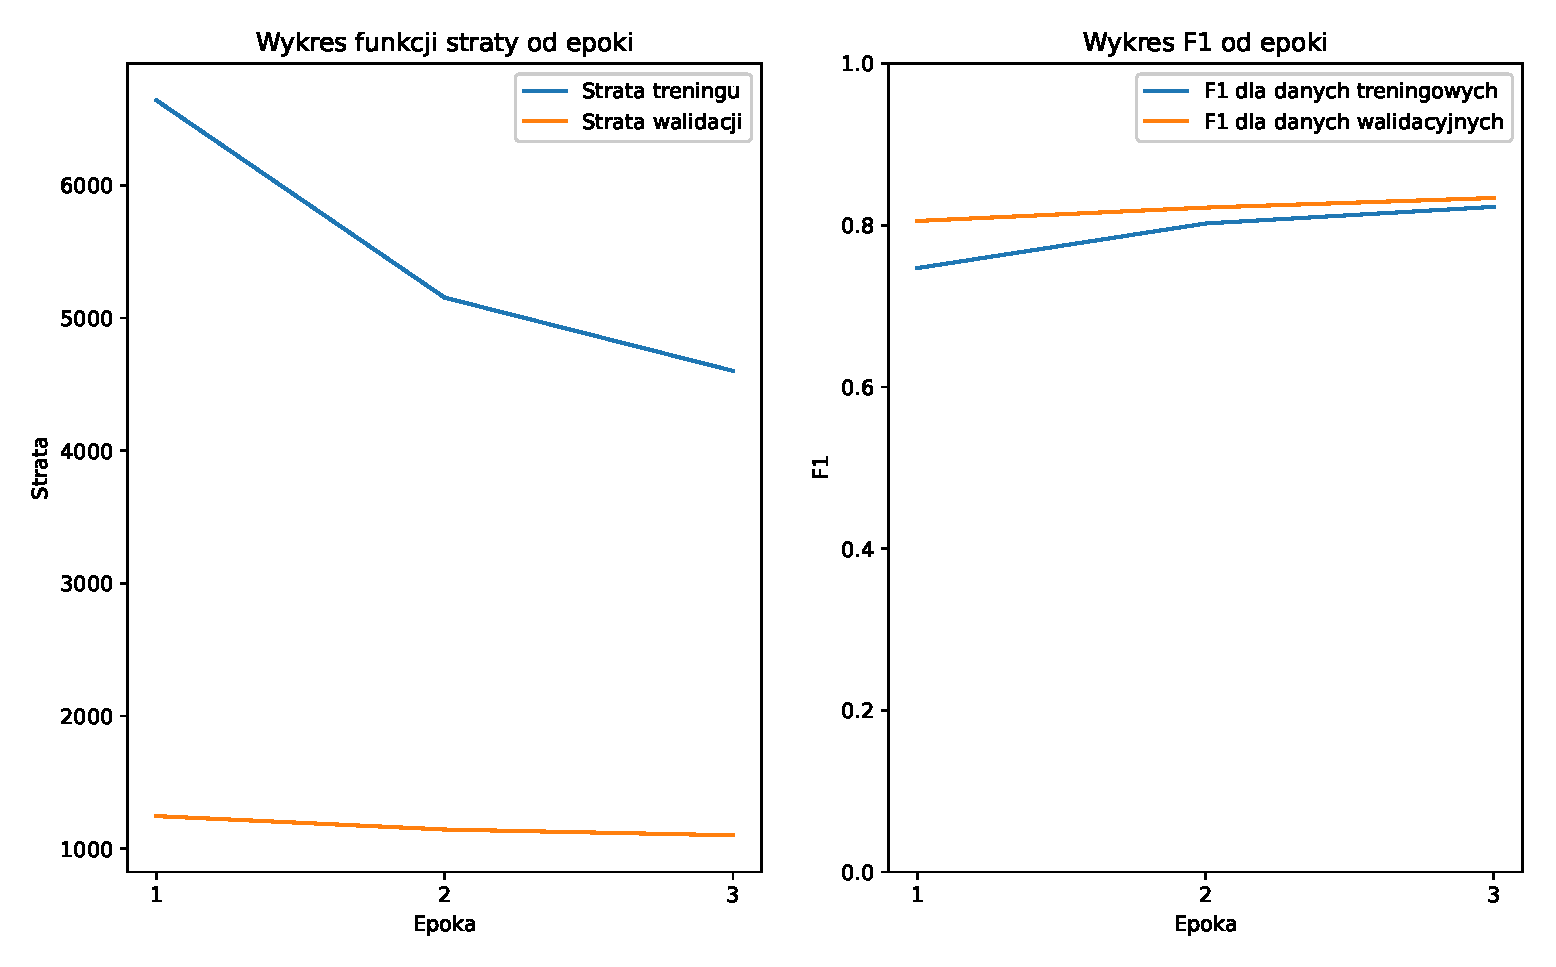
\includegraphics[width=\textwidth]{experiments/efficientnet_b0/combined}
    \caption{Wykres zależności funkcji straty i F1 od epoki trenowania}
    \label{fig:plot}
\end{figure}

\begin{figure}
    \centering
    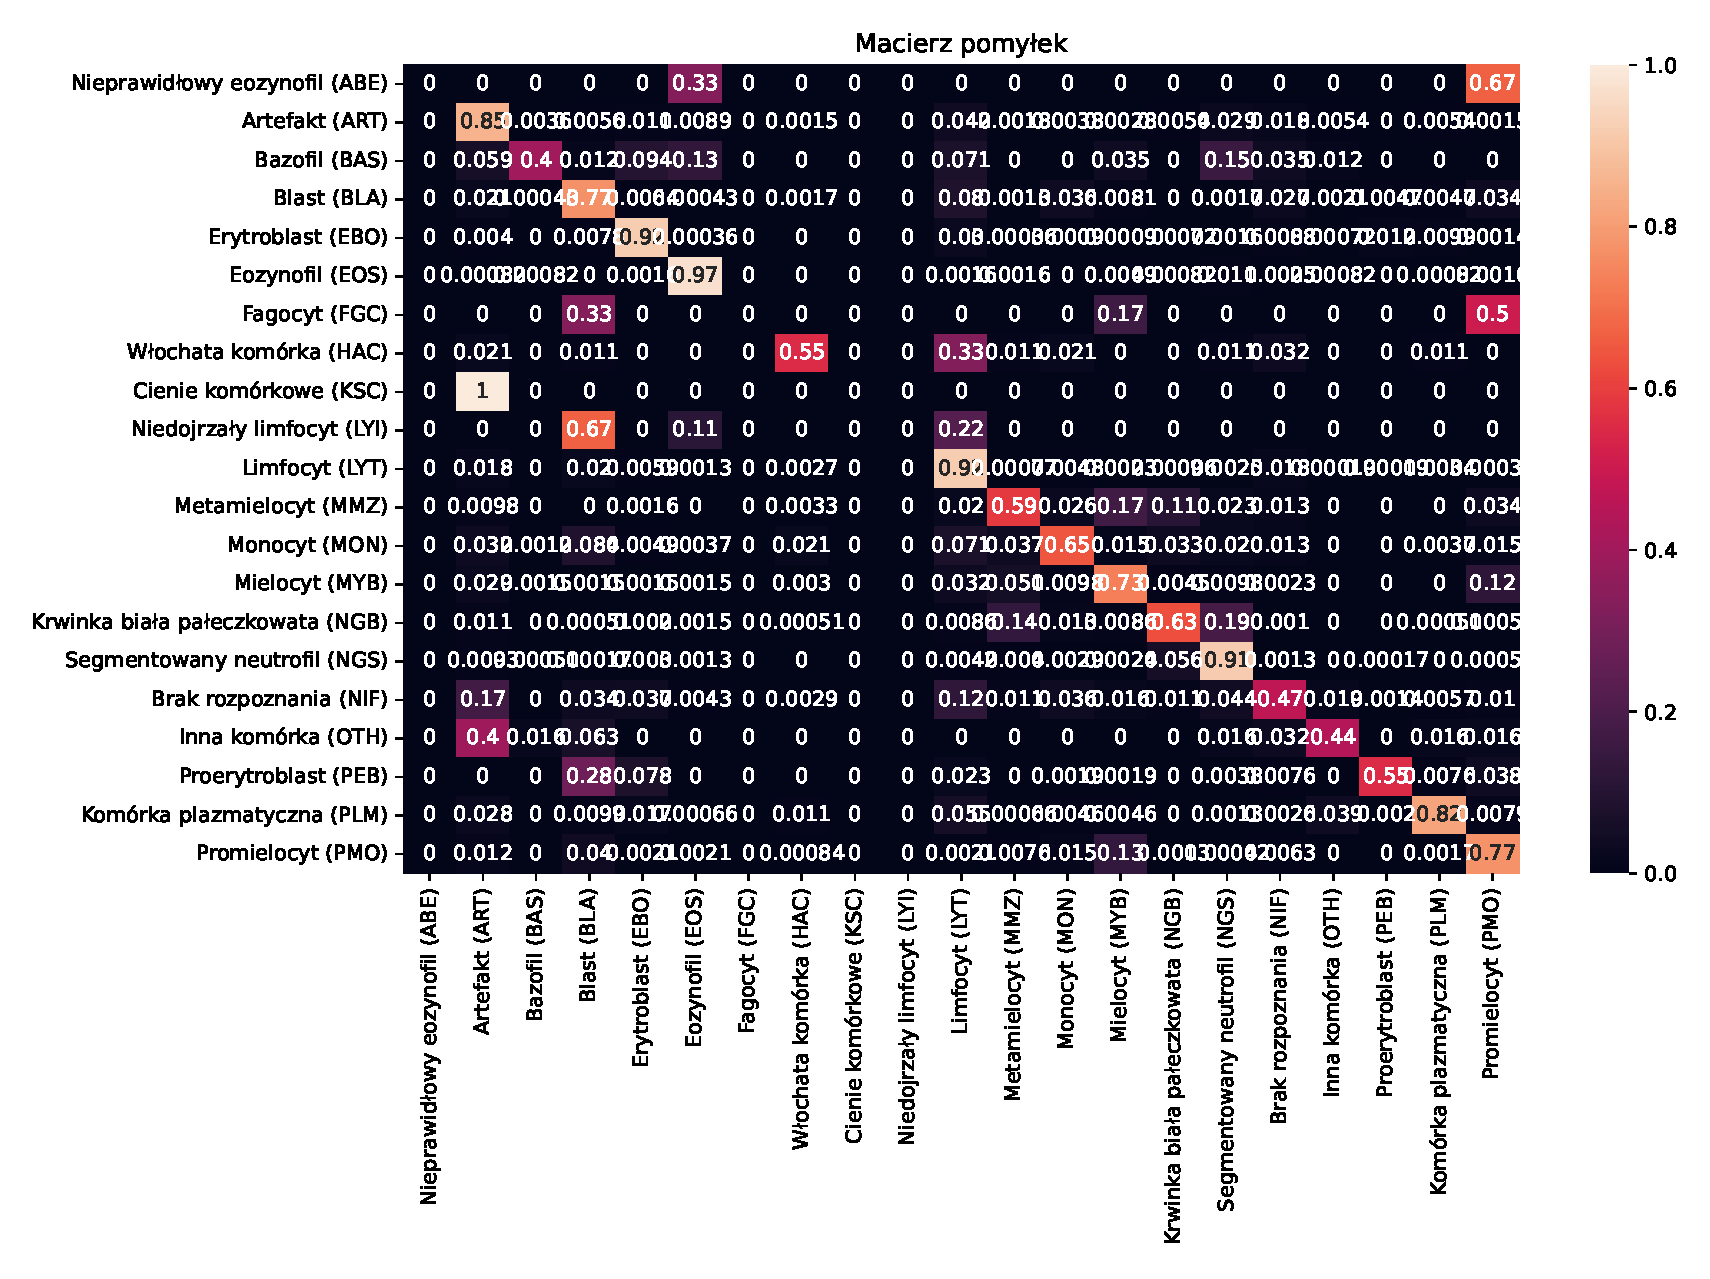
\includegraphics[width=\textwidth]{experiments/efficientnet_b0/confusion_matrix}
    \caption{Macierz pomyłek dla najlepszego modelu}
    \label{fig:confusion_matrix}
\end{figure}

%TODO start 9 listings

\begin{figure}
    \centering
    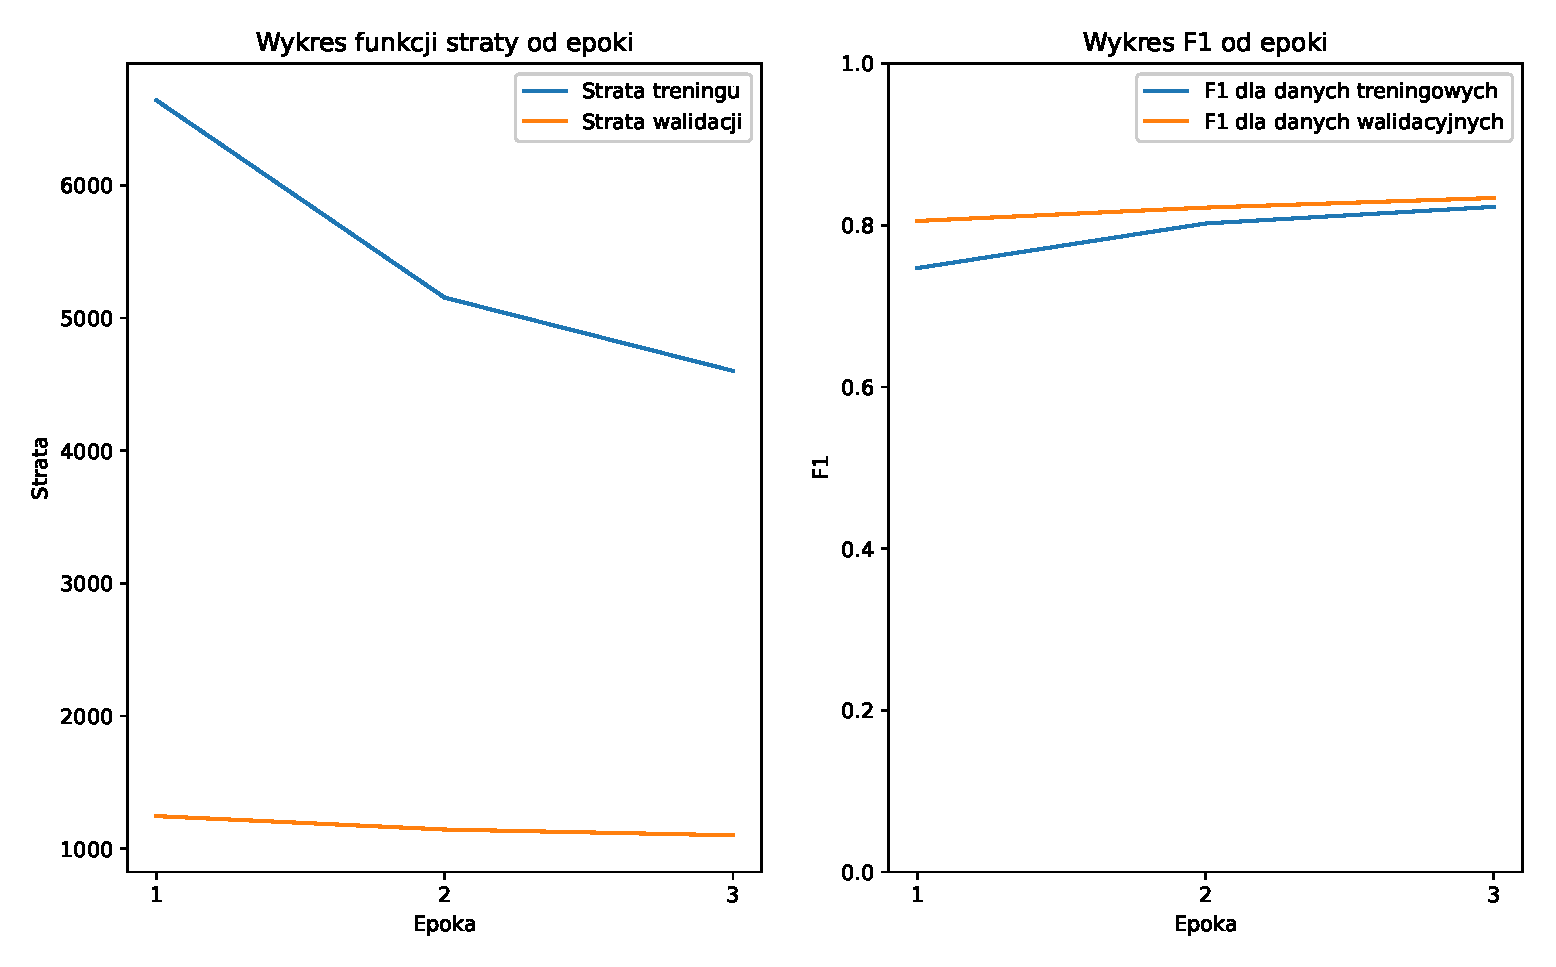
\includegraphics[width=\textwidth]{experiments/efficientnet_b0/combined}
    \caption{Wykres zależności funkcji straty i F1 od epoki trenowania}
\end{figure}

\begin{figure}
    \centering
    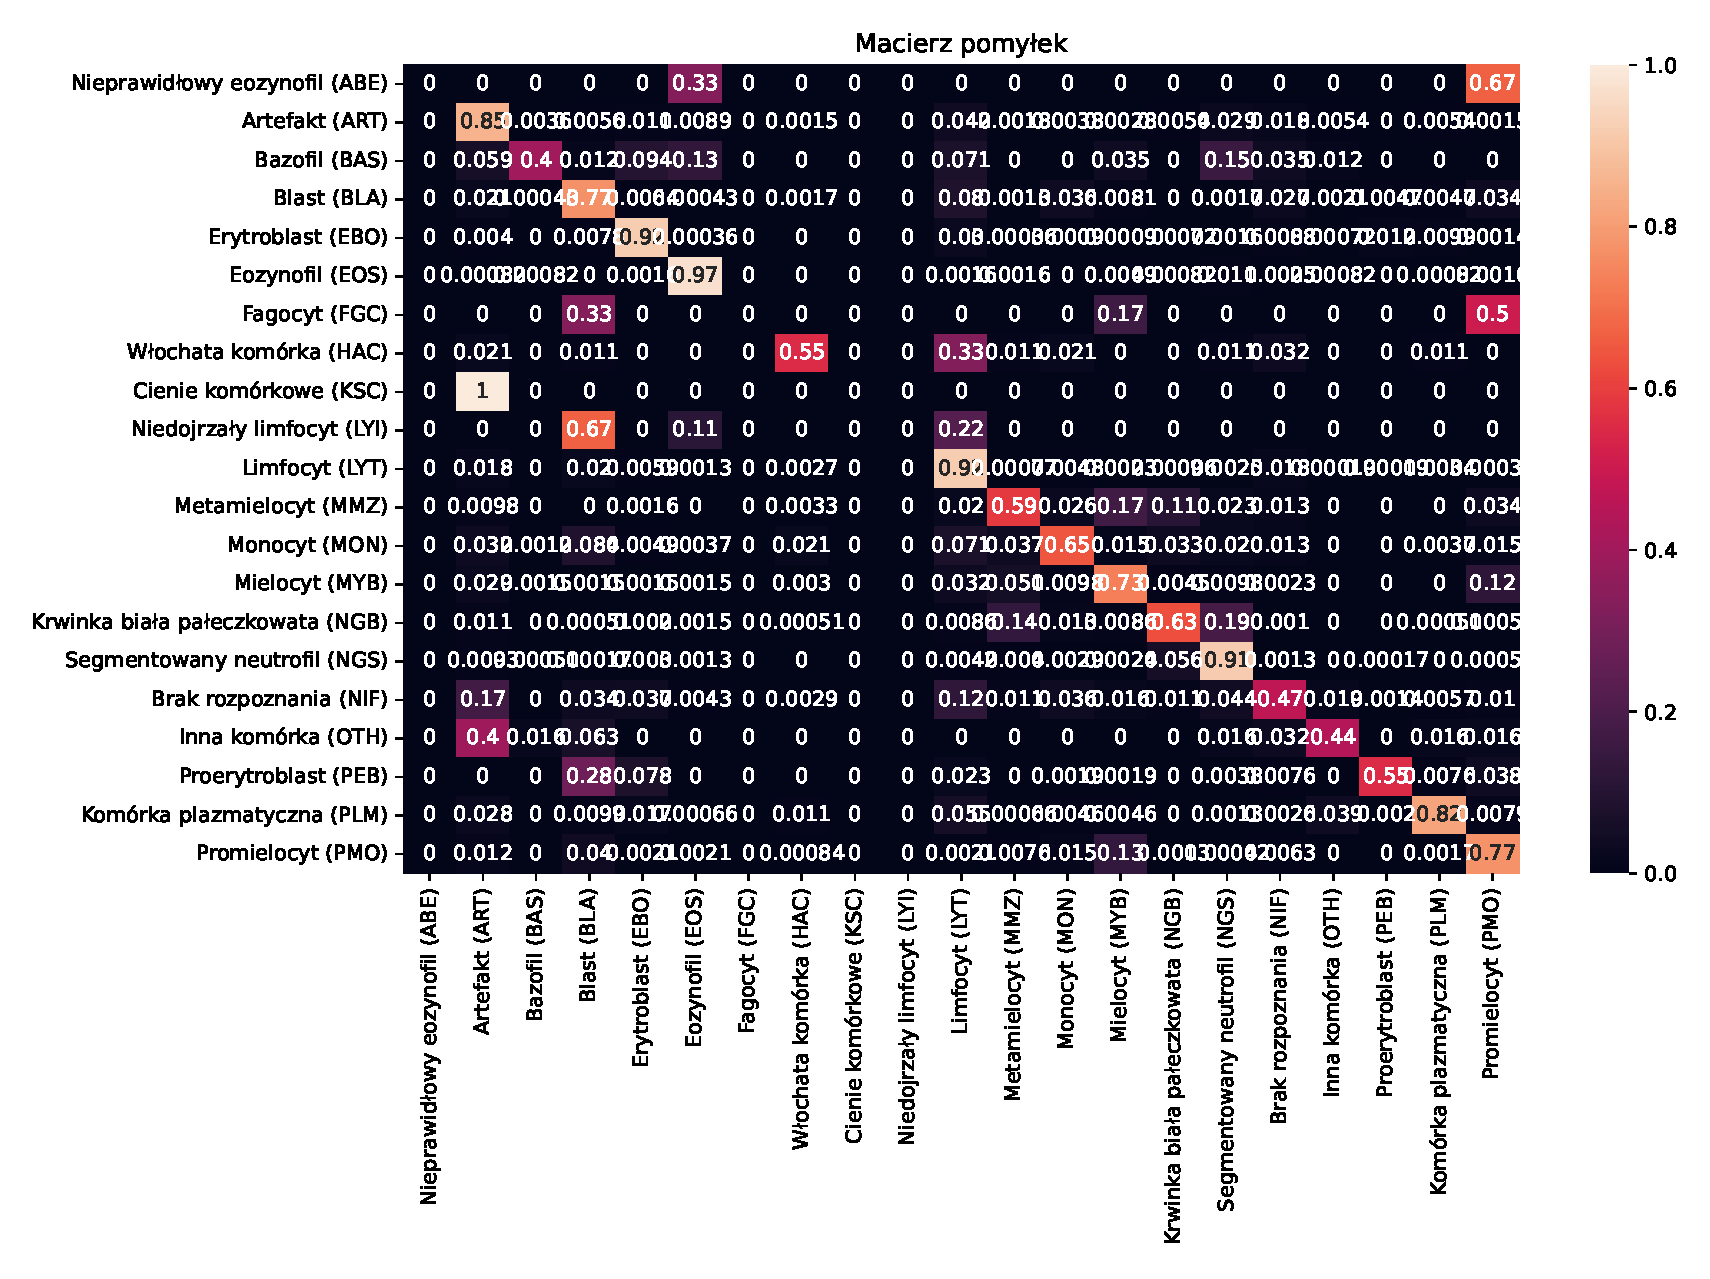
\includegraphics[width=\textwidth]{experiments/efficientnet_b0/confusion_matrix}
    \caption{Macierz pomyłek dla najlepszego modelu}
\end{figure}

\begin{figure}
    \centering
    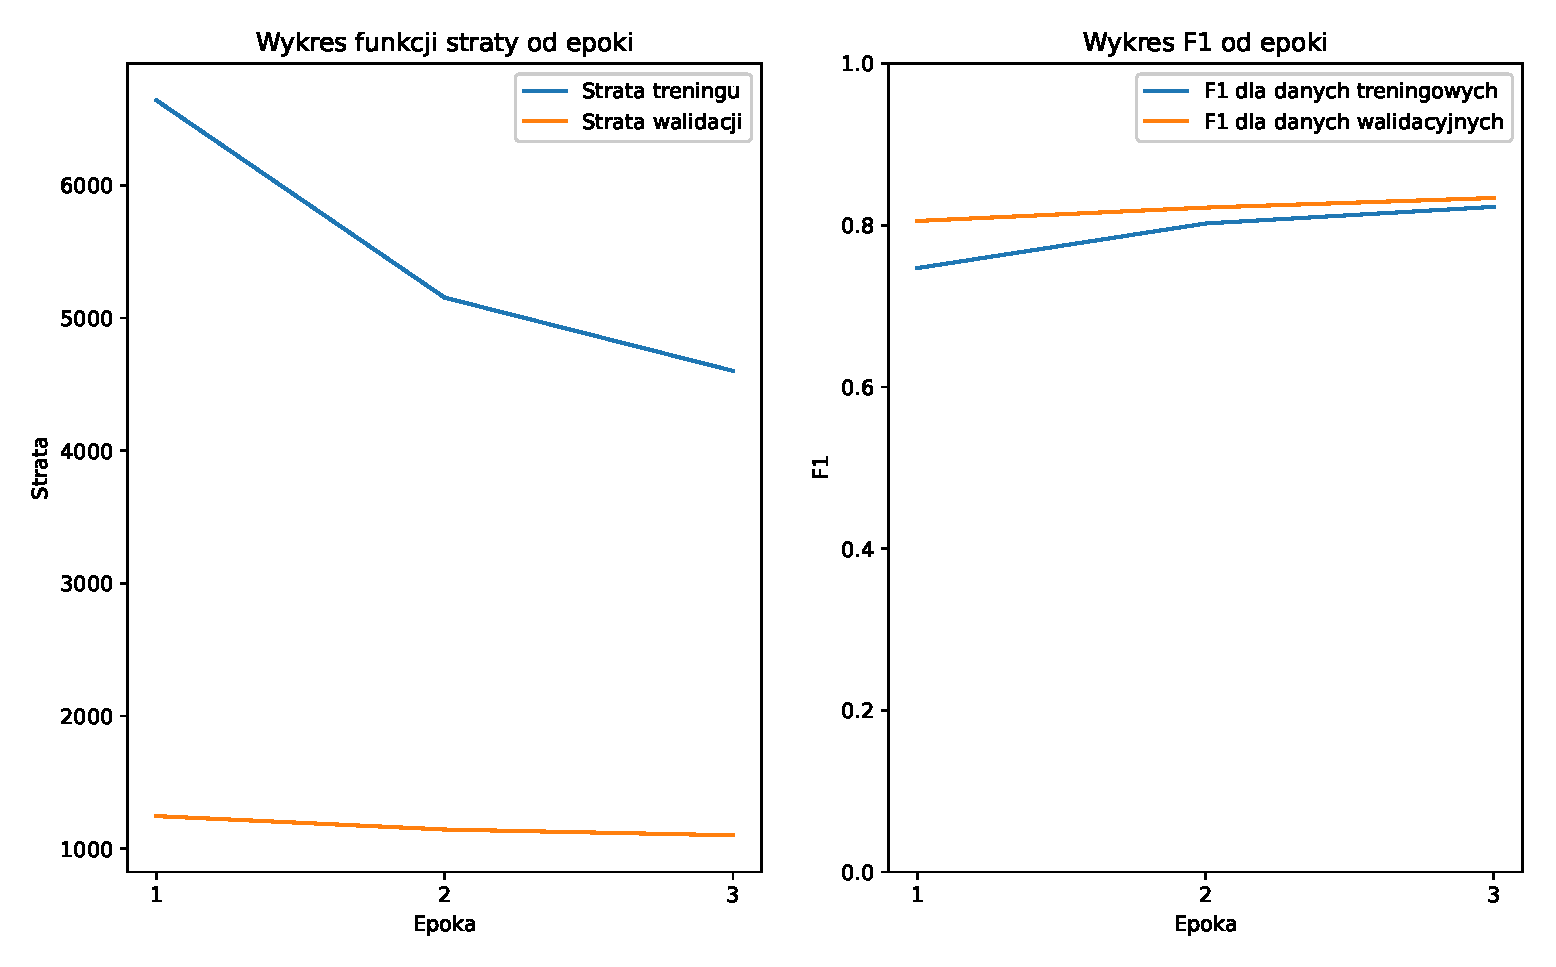
\includegraphics[width=\textwidth]{experiments/efficientnet_b0/combined}
    \caption{Wykres zależności funkcji straty i F1 od epoki trenowania}
\end{figure}

\begin{figure}
    \centering
    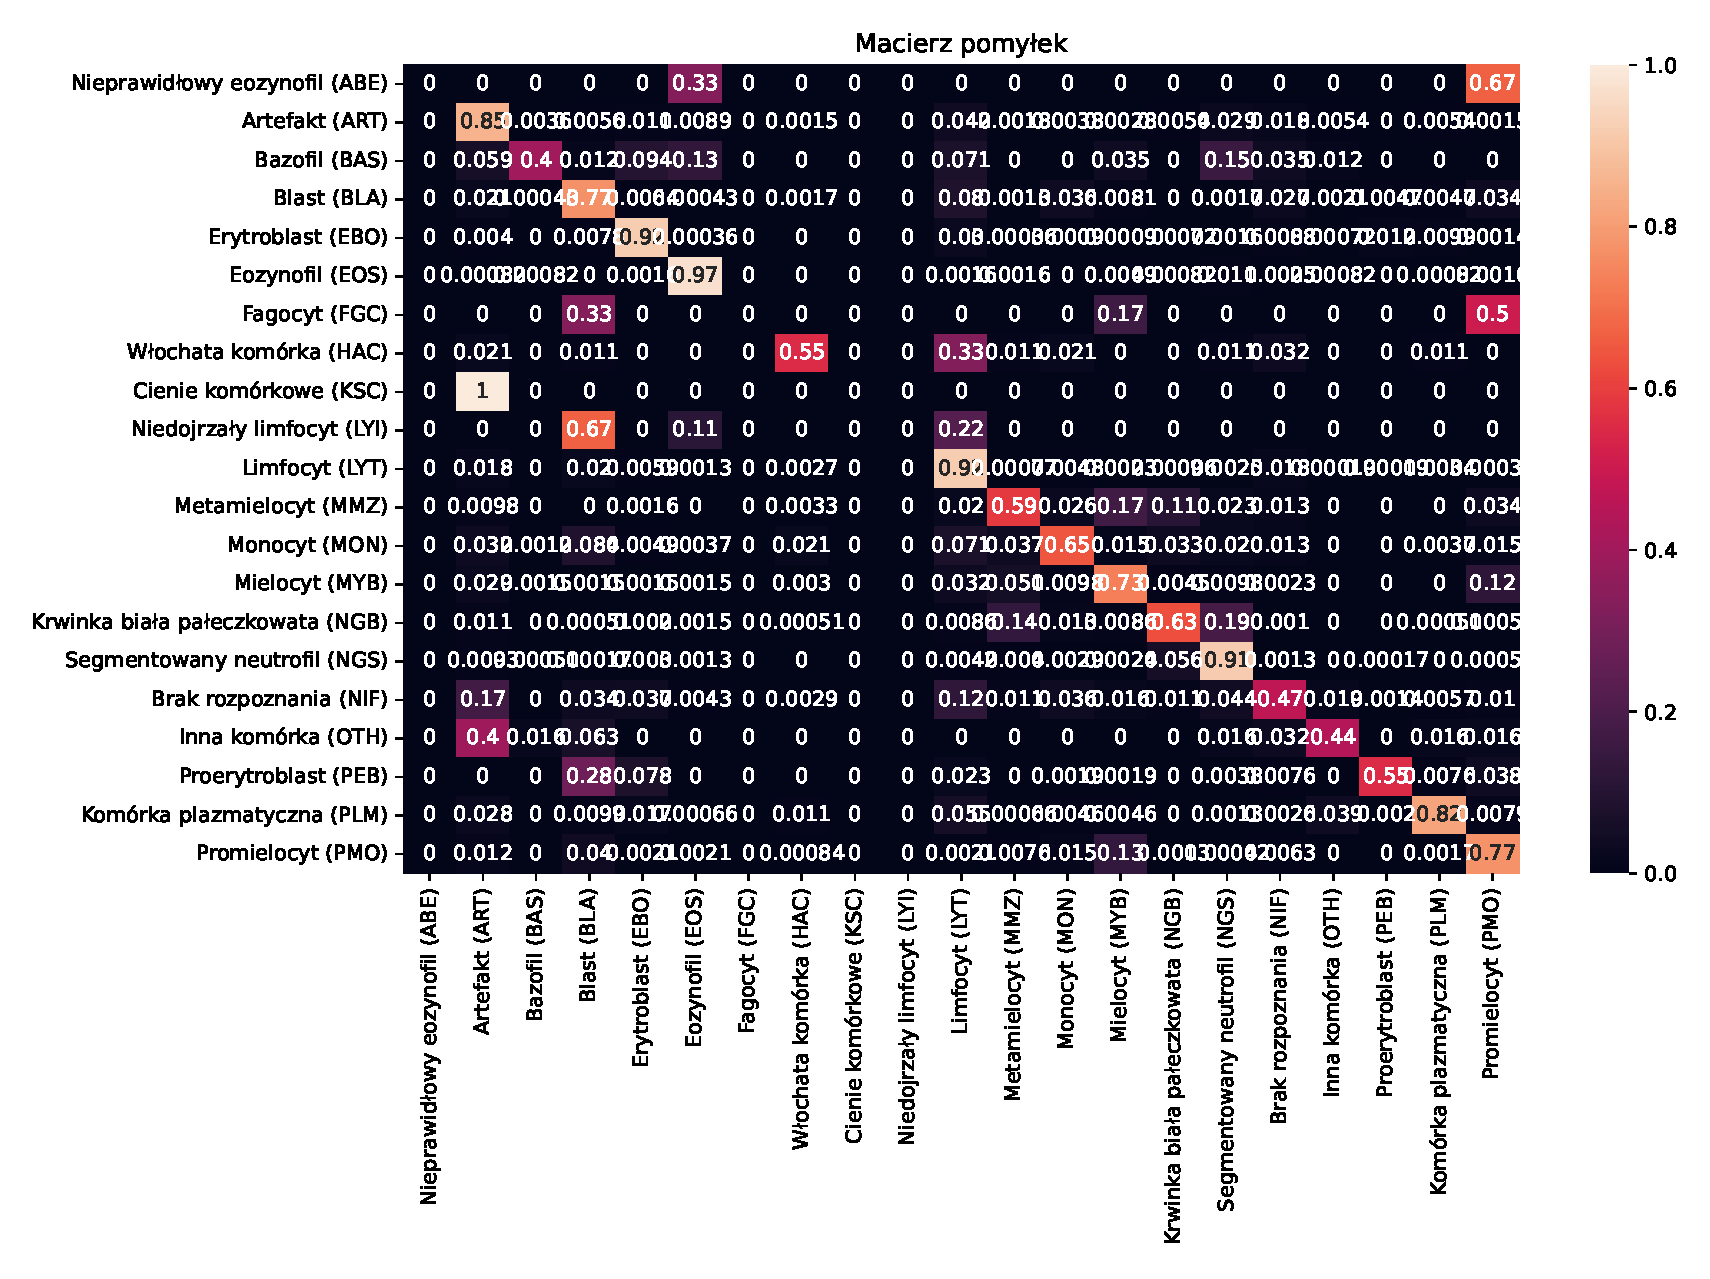
\includegraphics[width=\textwidth]{experiments/efficientnet_b0/confusion_matrix}
    \caption{Macierz pomyłek dla najlepszego modelu}
\end{figure}

\begin{figure}
    \centering
    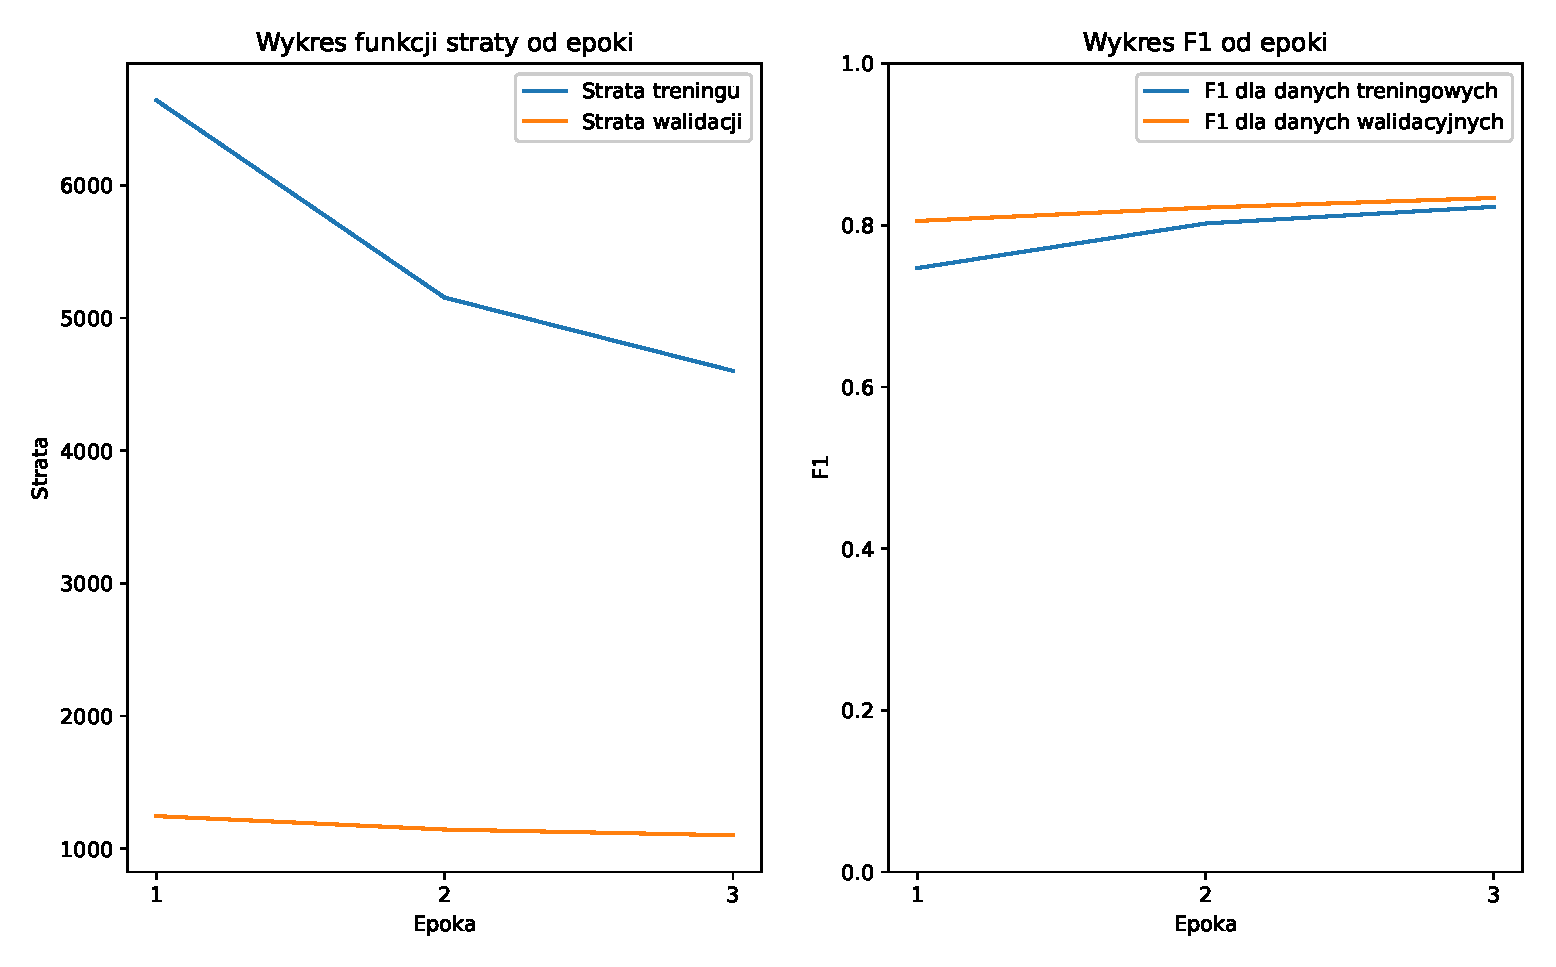
\includegraphics[width=\textwidth]{experiments/efficientnet_b0/combined}
    \caption{Wykres zależności funkcji straty i F1 od epoki trenowania}
\end{figure}

\begin{figure}
    \centering
    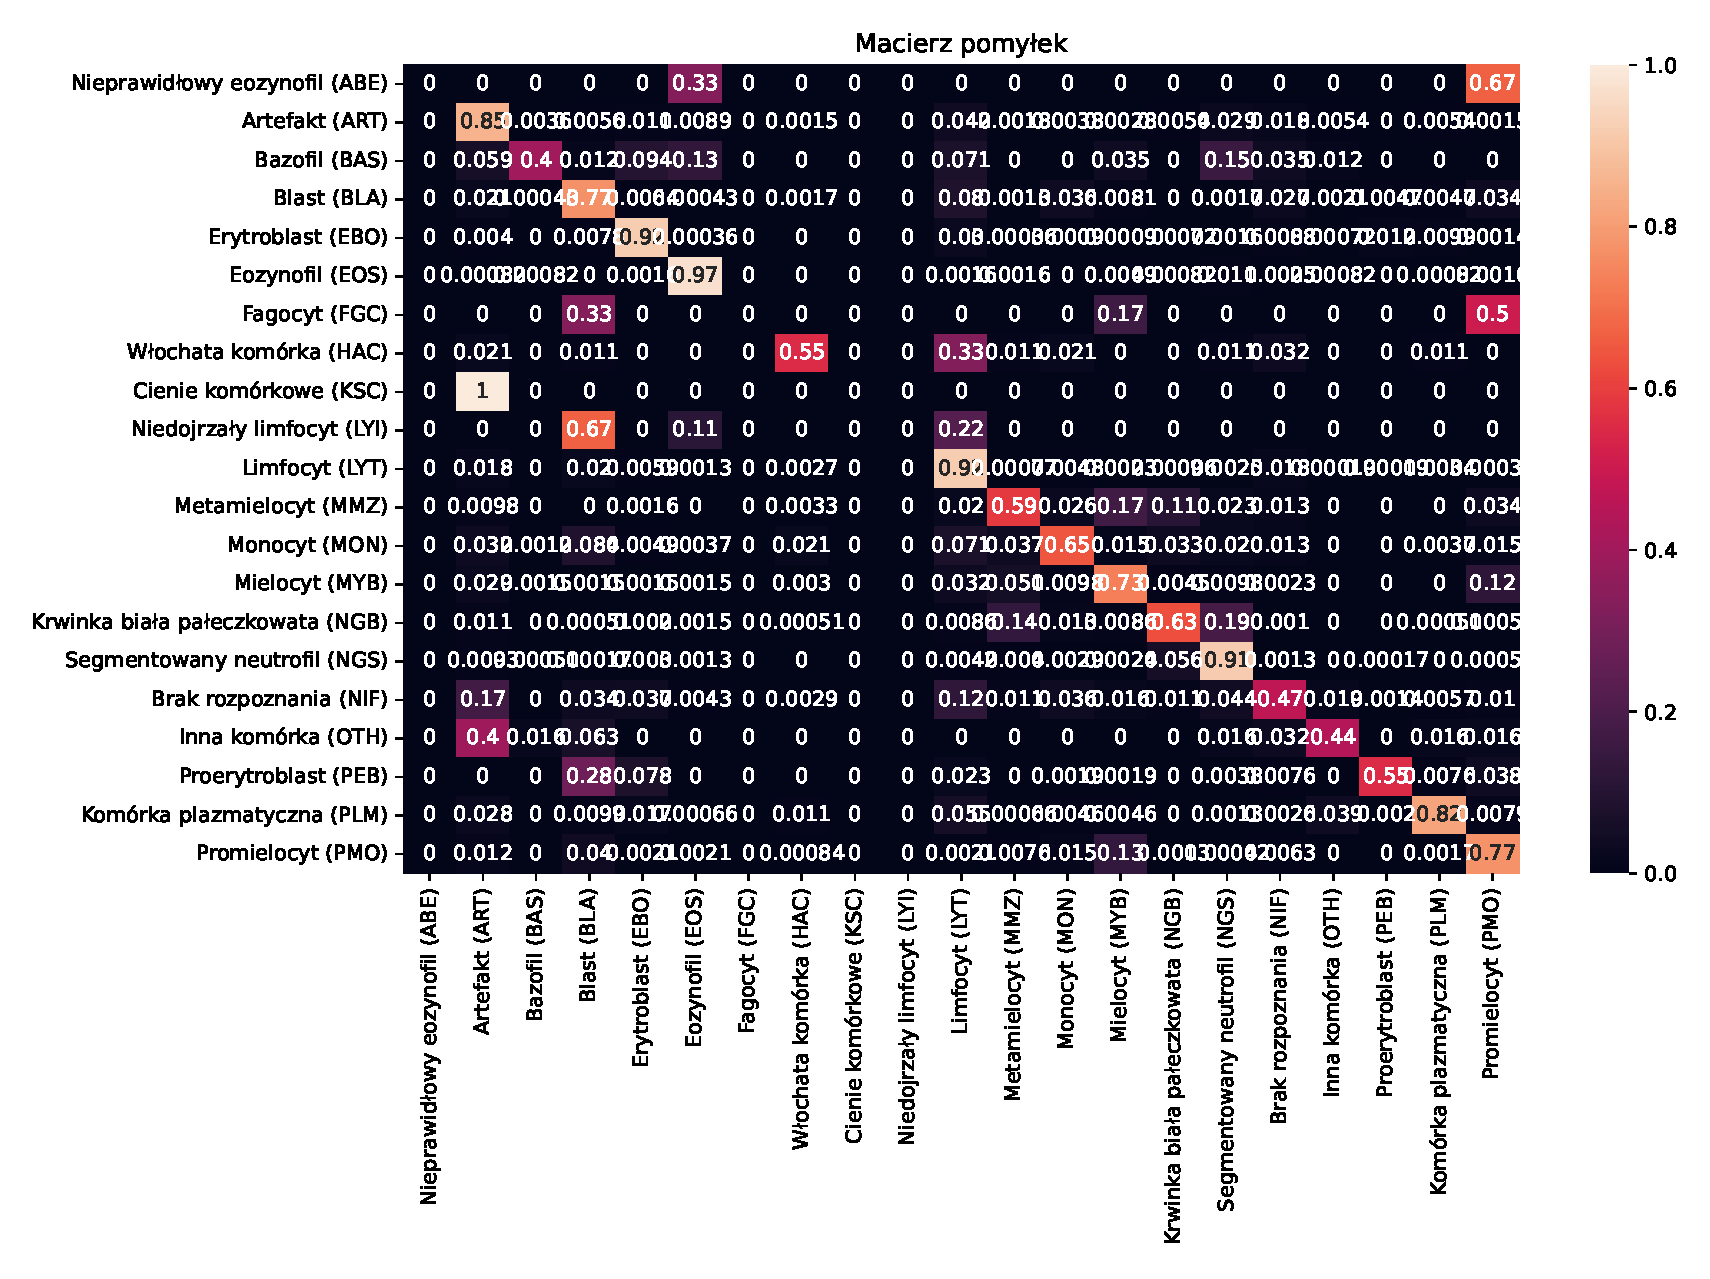
\includegraphics[width=\textwidth]{experiments/efficientnet_b0/confusion_matrix}
    \caption{Macierz pomyłek dla najlepszego modelu}
\end{figure}

\begin{figure}
    \centering
    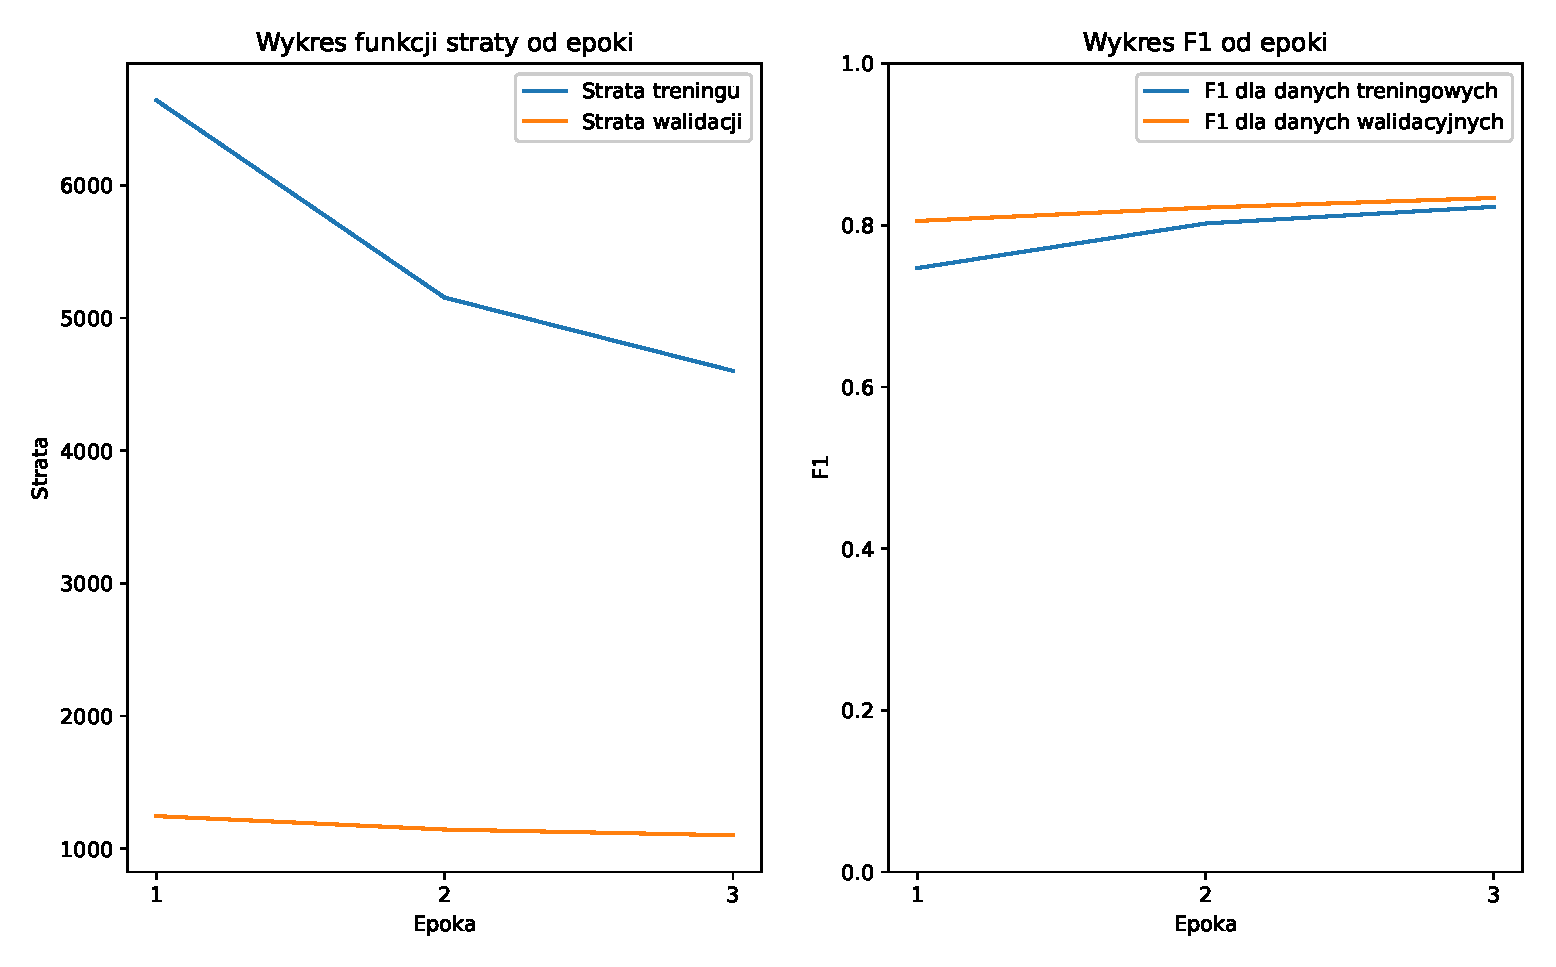
\includegraphics[width=\textwidth]{experiments/efficientnet_b0/combined}
    \caption{Wykres zależności funkcji straty i F1 od epoki trenowania}
\end{figure}

\begin{figure}
    \centering
    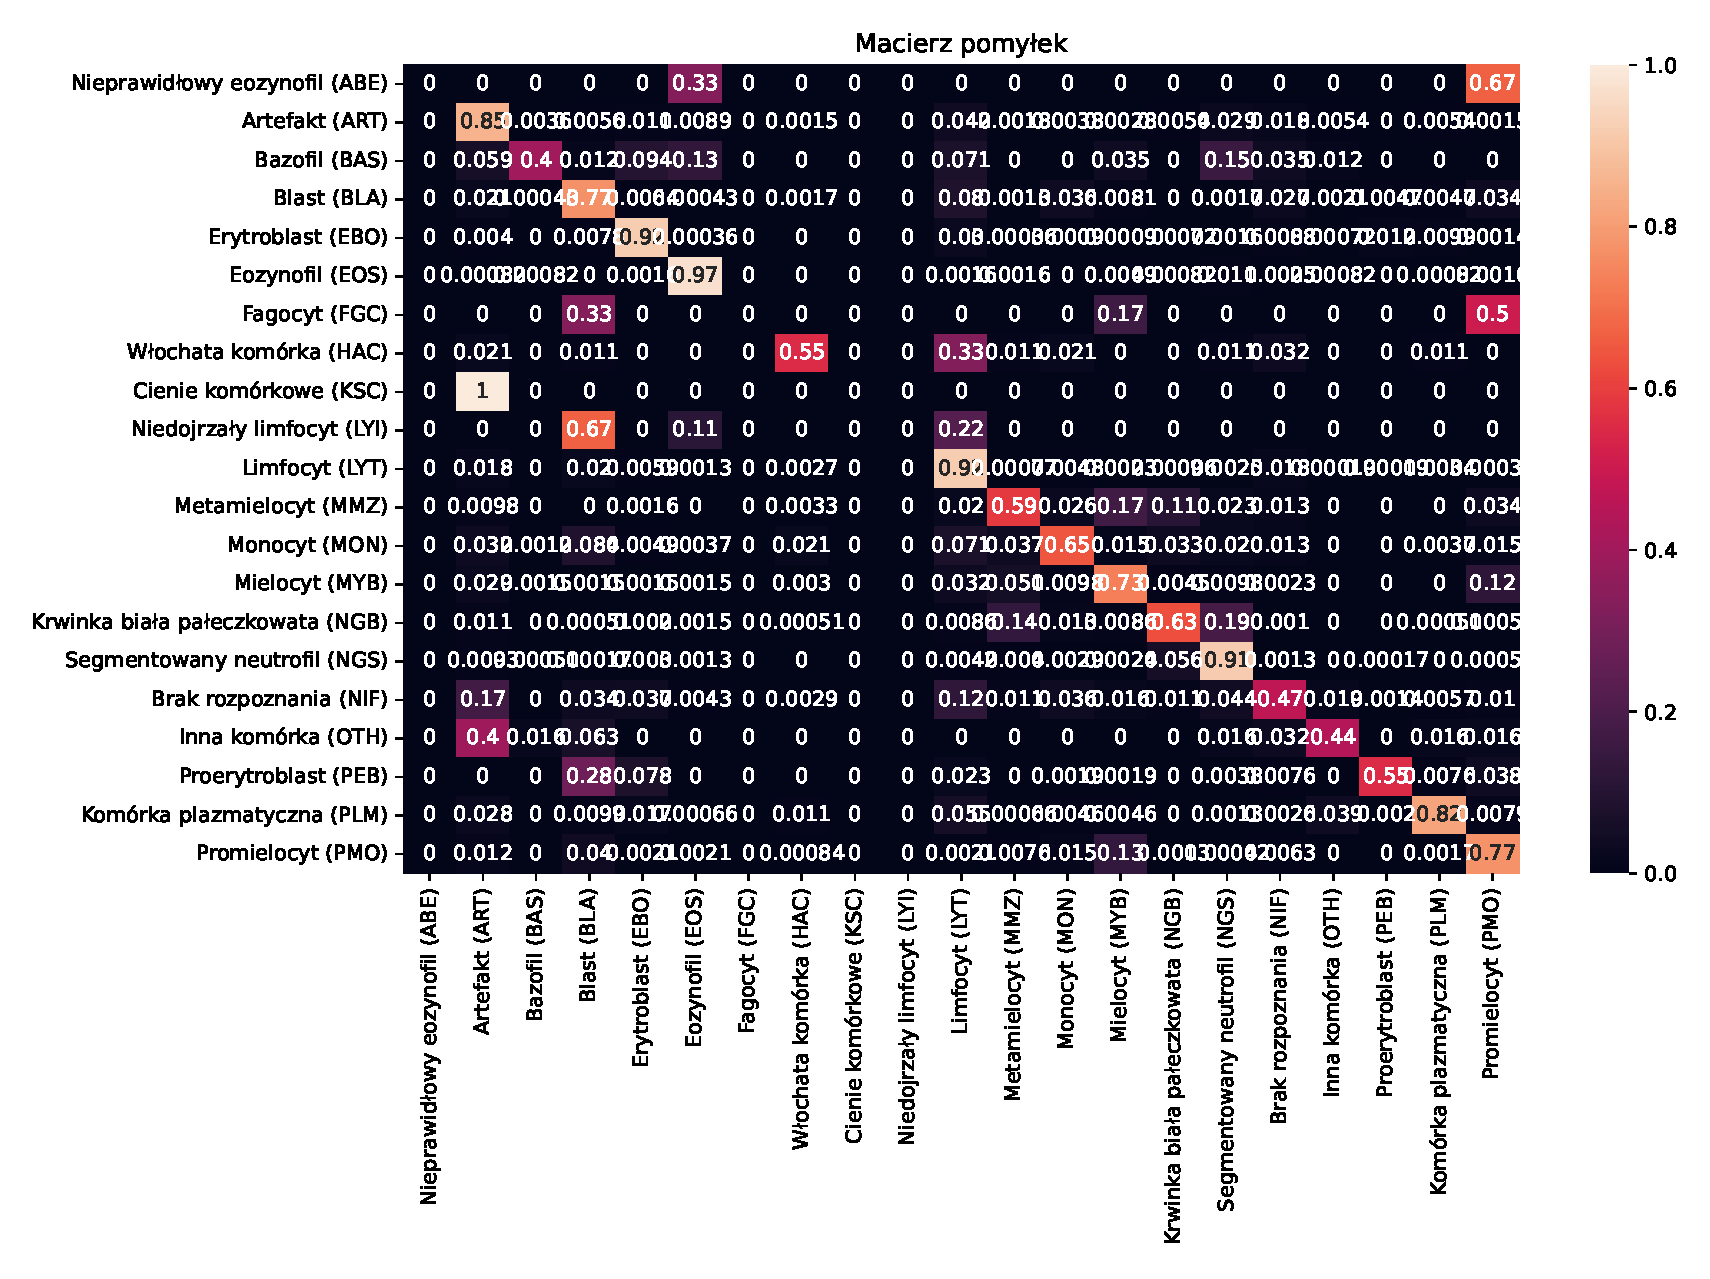
\includegraphics[width=\textwidth]{experiments/efficientnet_b0/confusion_matrix}
    \caption{Macierz pomyłek dla najlepszego modelu}
\end{figure}

\begin{figure}
    \centering
    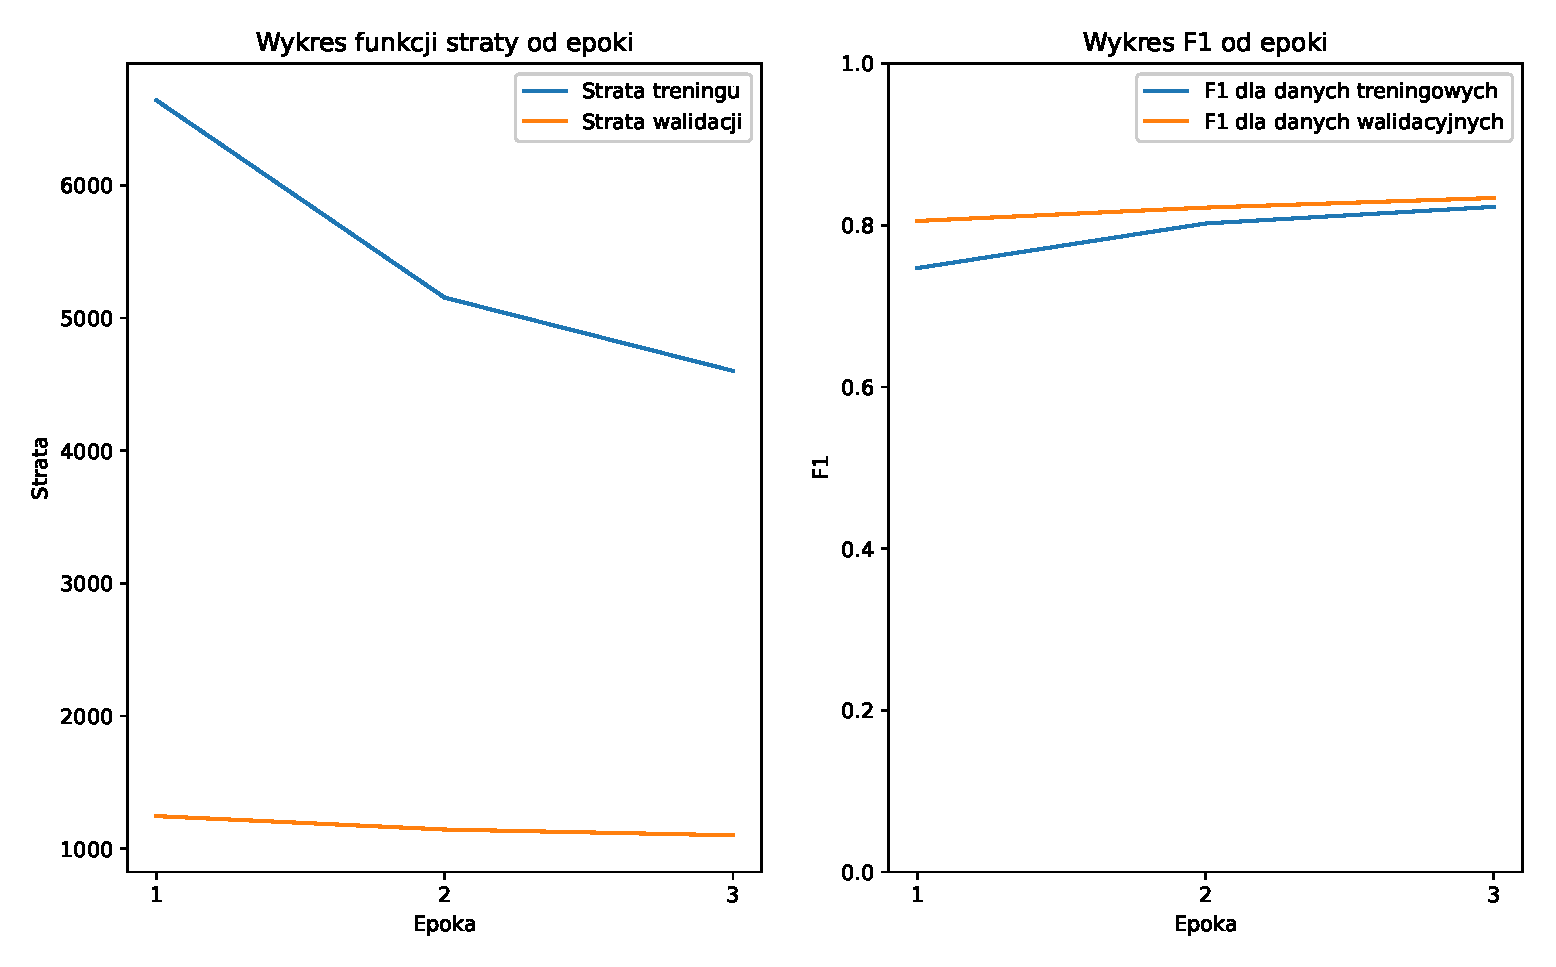
\includegraphics[width=\textwidth]{experiments/efficientnet_b0/combined}
    \caption{Wykres zależności funkcji straty i F1 od epoki trenowania}
\end{figure}

\begin{figure}
    \centering
    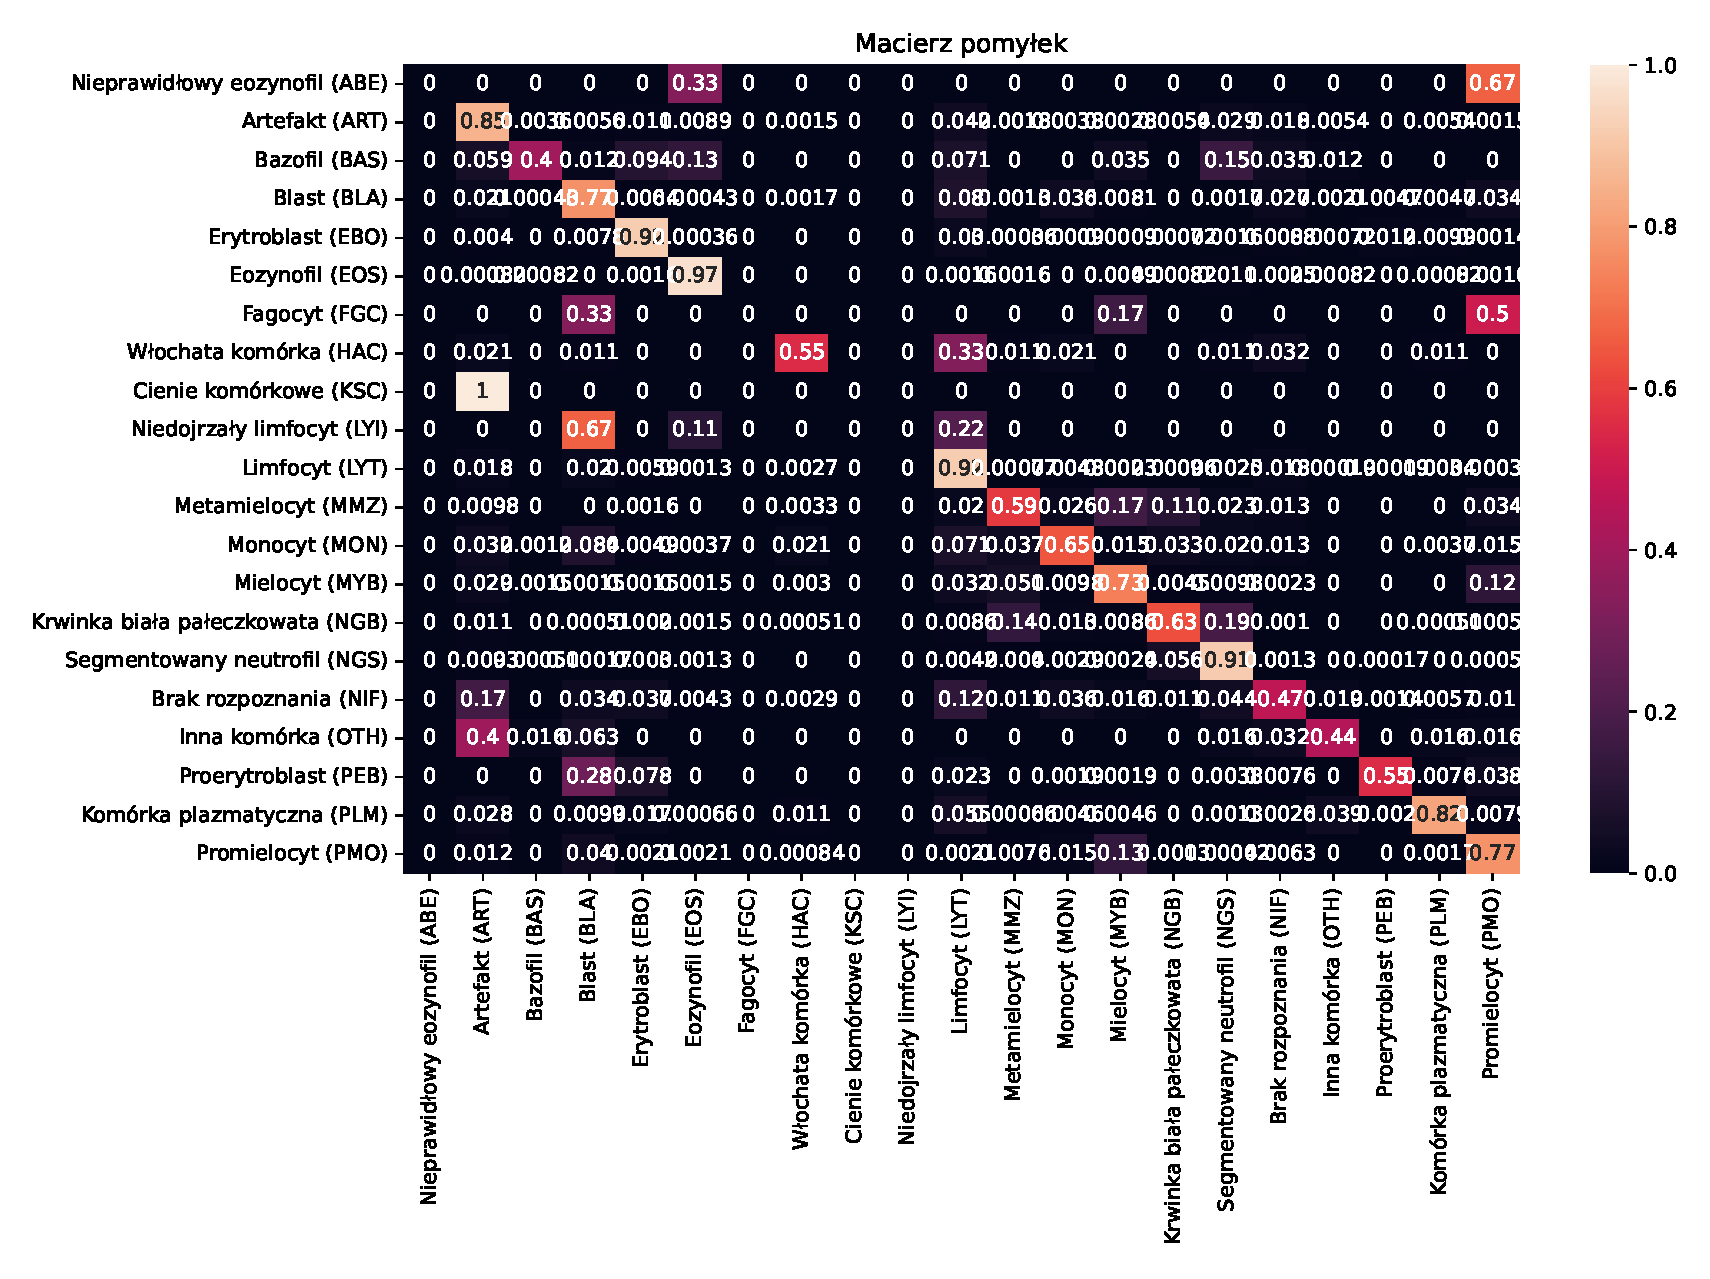
\includegraphics[width=\textwidth]{experiments/efficientnet_b0/confusion_matrix}
    \caption{Macierz pomyłek dla najlepszego modelu}
\end{figure}

\begin{figure}
    \centering
    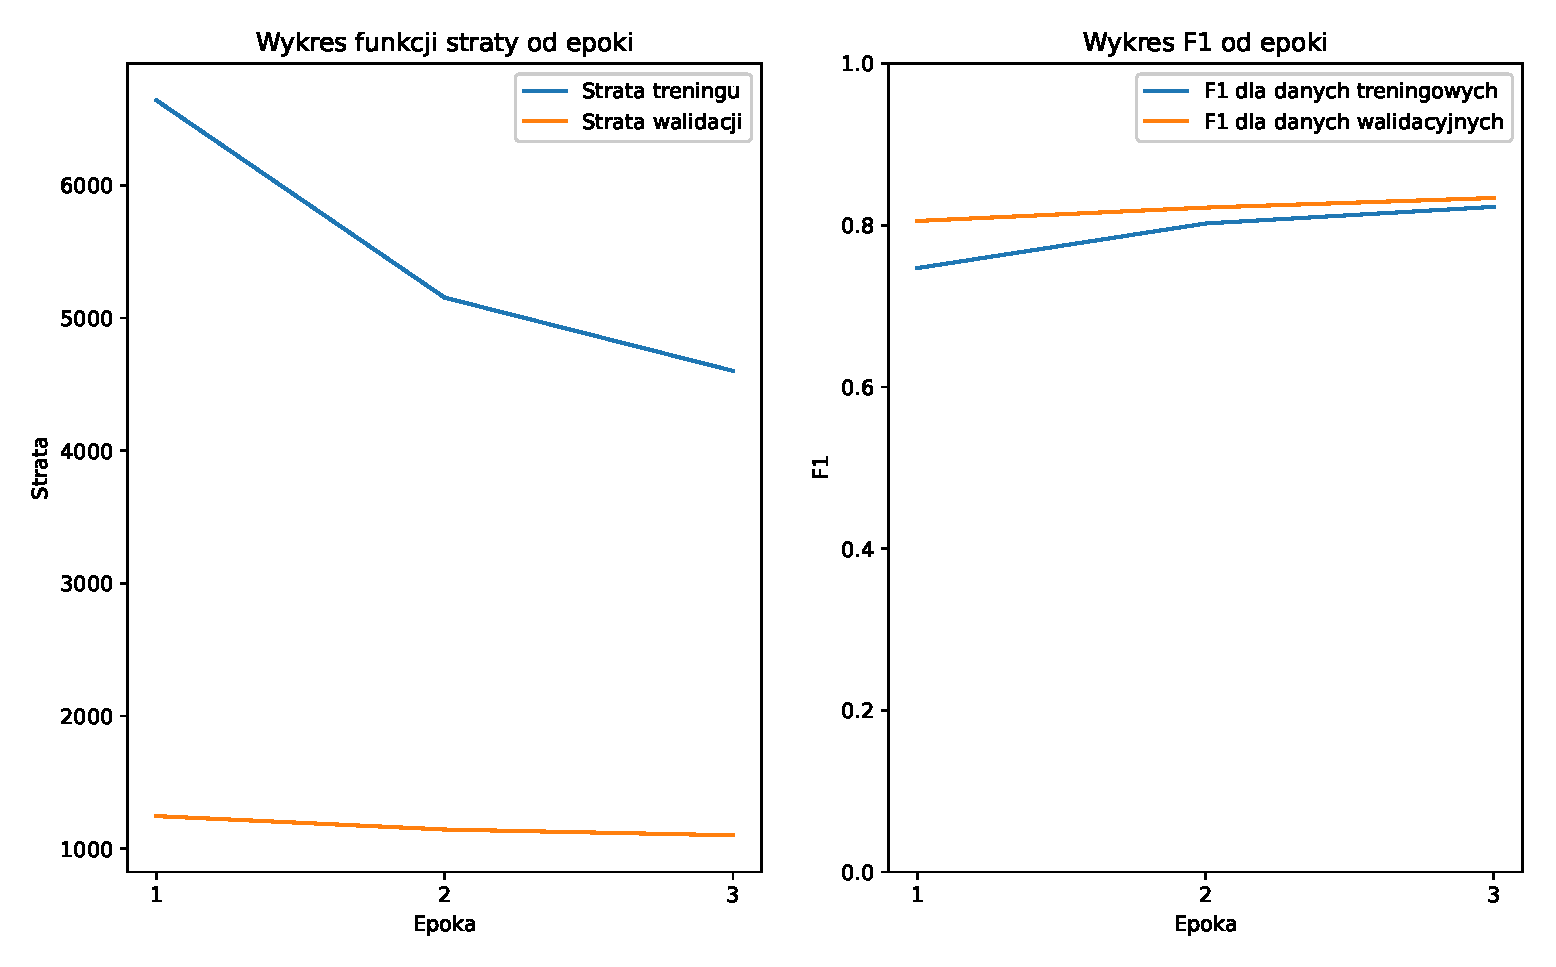
\includegraphics[width=\textwidth]{experiments/efficientnet_b0/combined}
    \caption{Wykres zależności funkcji straty i F1 od epoki trenowania}
\end{figure}

\begin{figure}
    \centering
    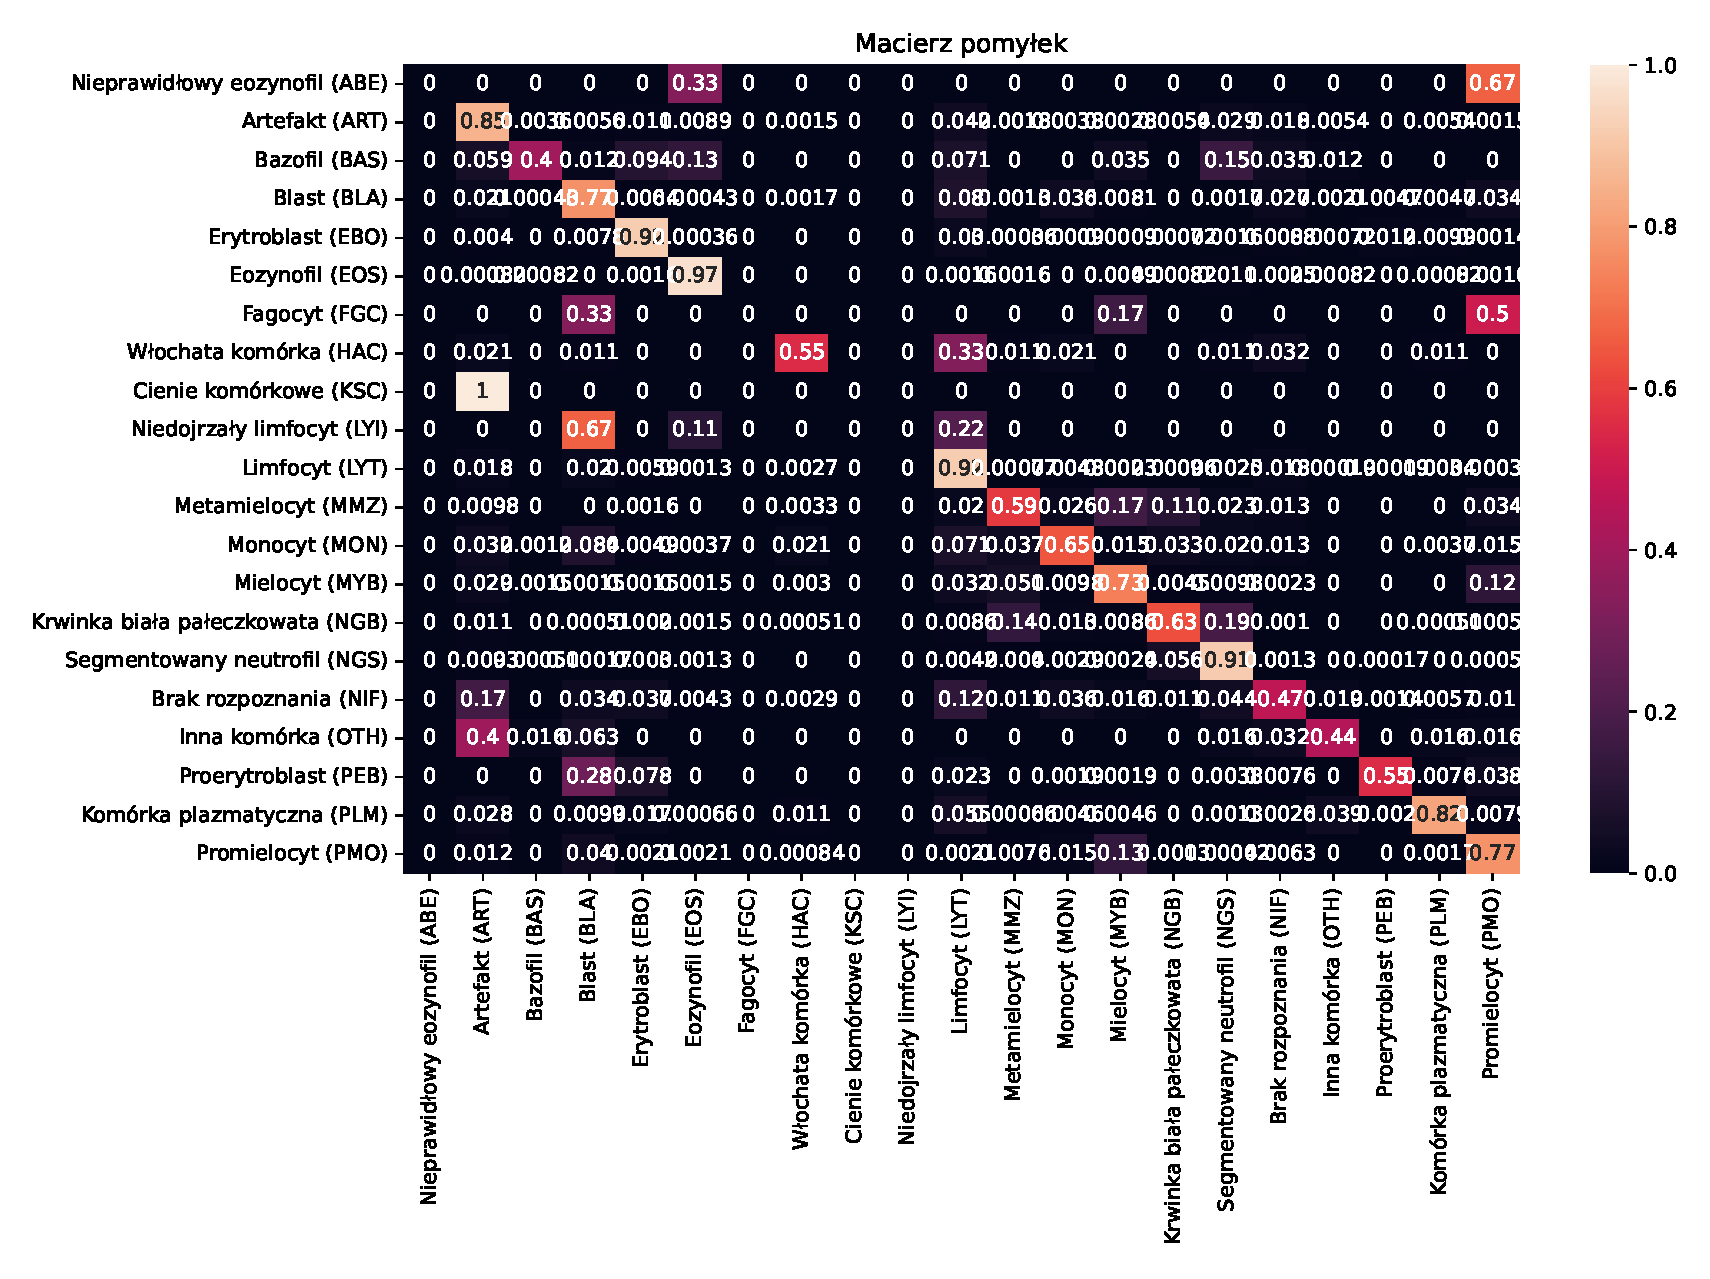
\includegraphics[width=\textwidth]{experiments/efficientnet_b0/confusion_matrix}
    \caption{Macierz pomyłek dla najlepszego modelu}
\end{figure}

\begin{figure}
    \centering
    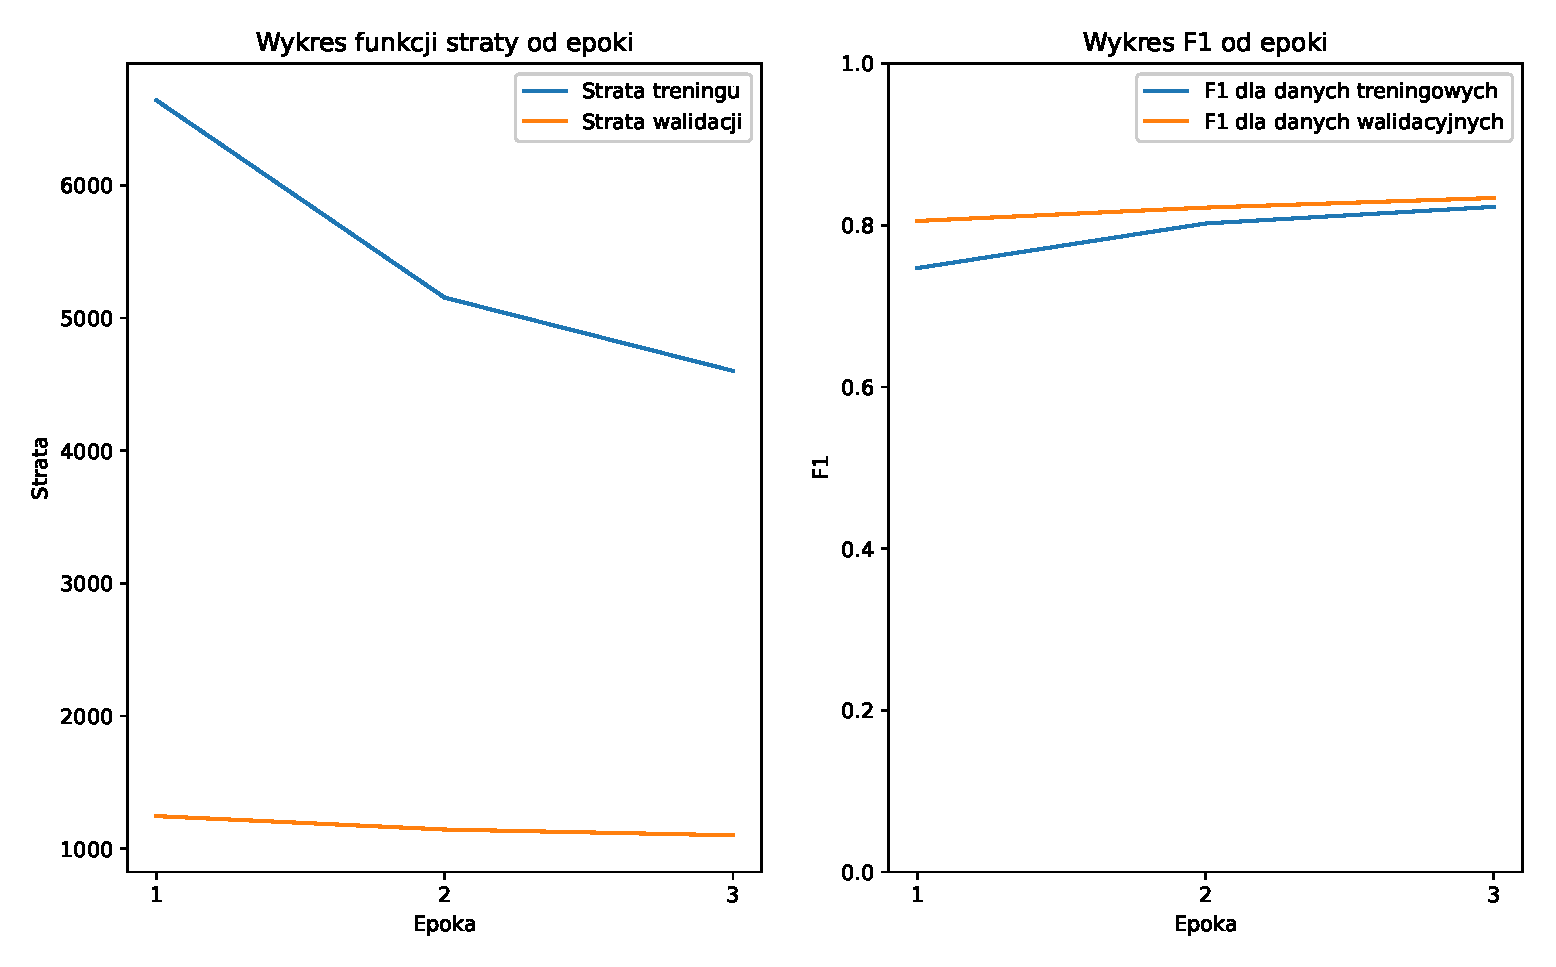
\includegraphics[width=\textwidth]{experiments/efficientnet_b0/combined}
    \caption{Wykres zależności funkcji straty i F1 od epoki trenowania}
\end{figure}

\begin{figure}
    \centering
    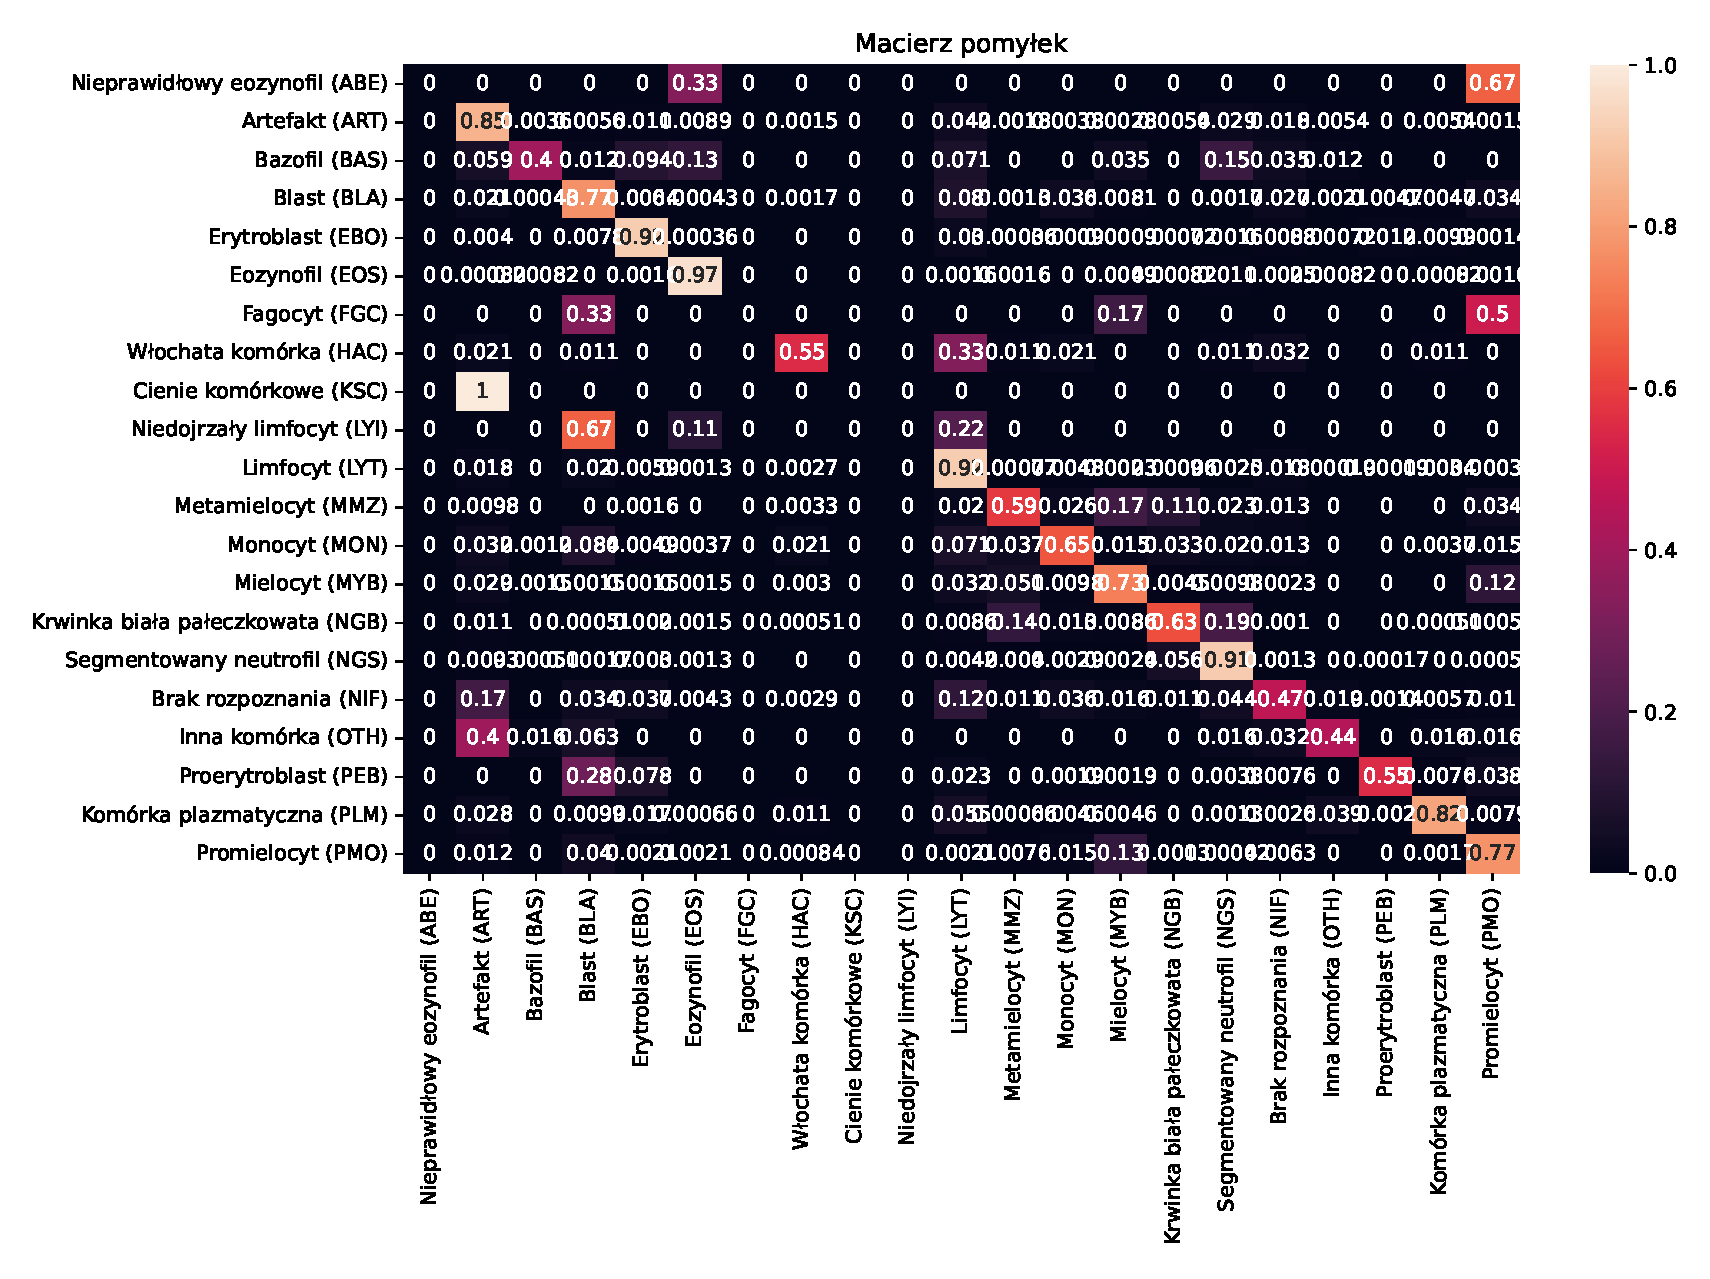
\includegraphics[width=\textwidth]{experiments/efficientnet_b0/confusion_matrix}
    \caption{Macierz pomyłek dla najlepszego modelu}
\end{figure}

\begin{figure}
    \centering
    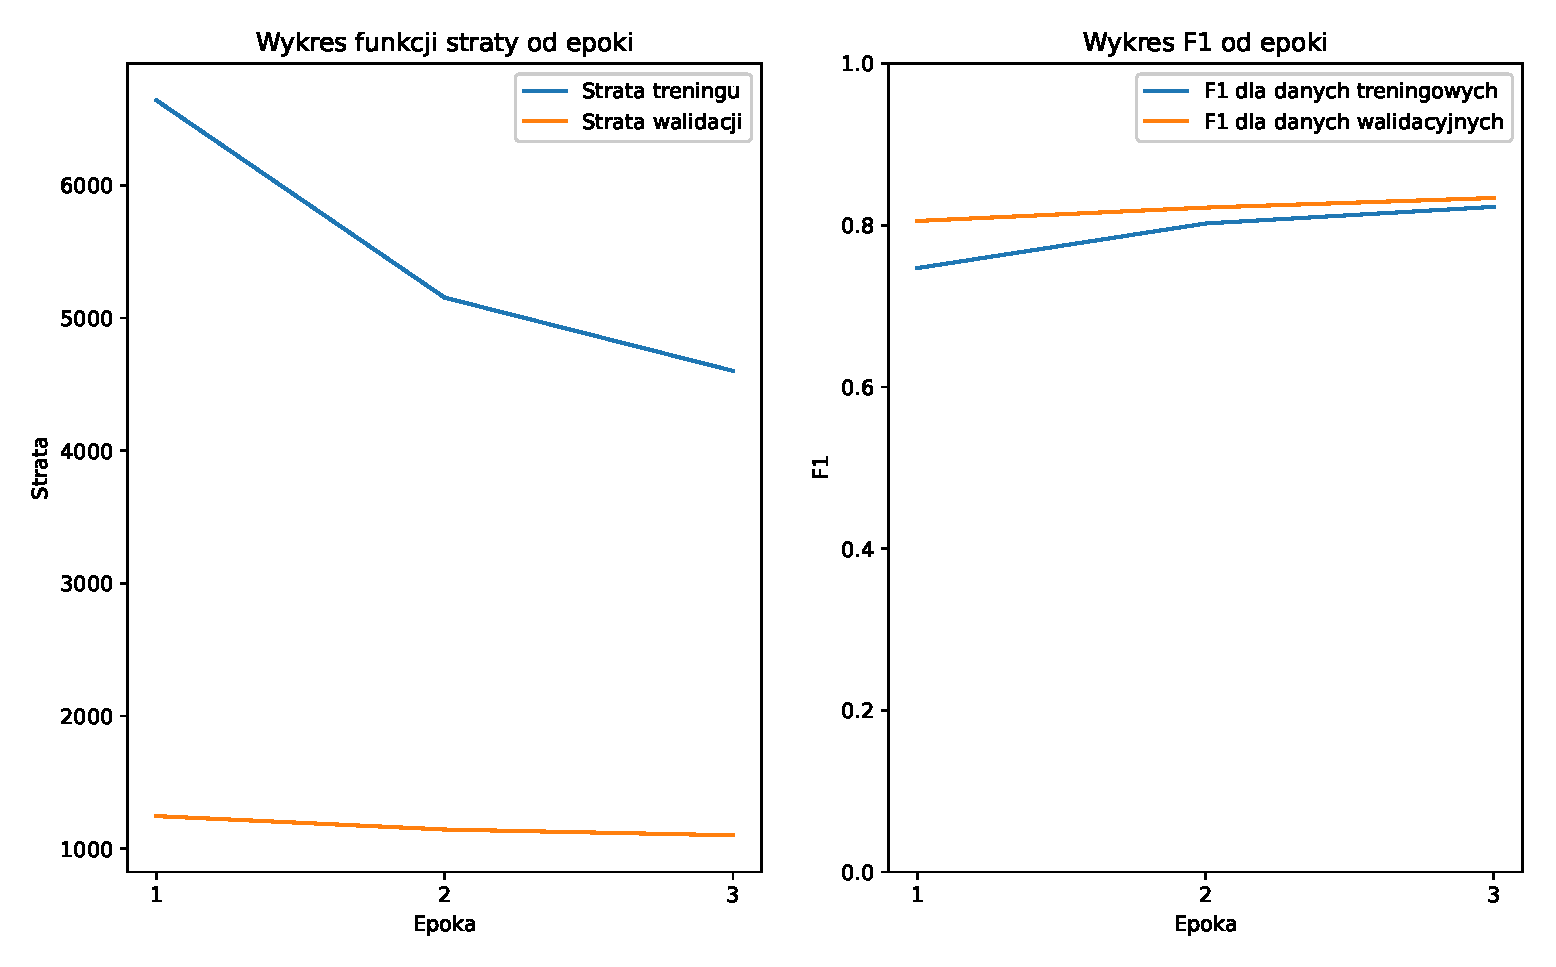
\includegraphics[width=\textwidth]{experiments/efficientnet_b0/combined}
    \caption{Wykres zależności funkcji straty i F1 od epoki trenowania}
\end{figure}

\begin{figure}
    \centering
    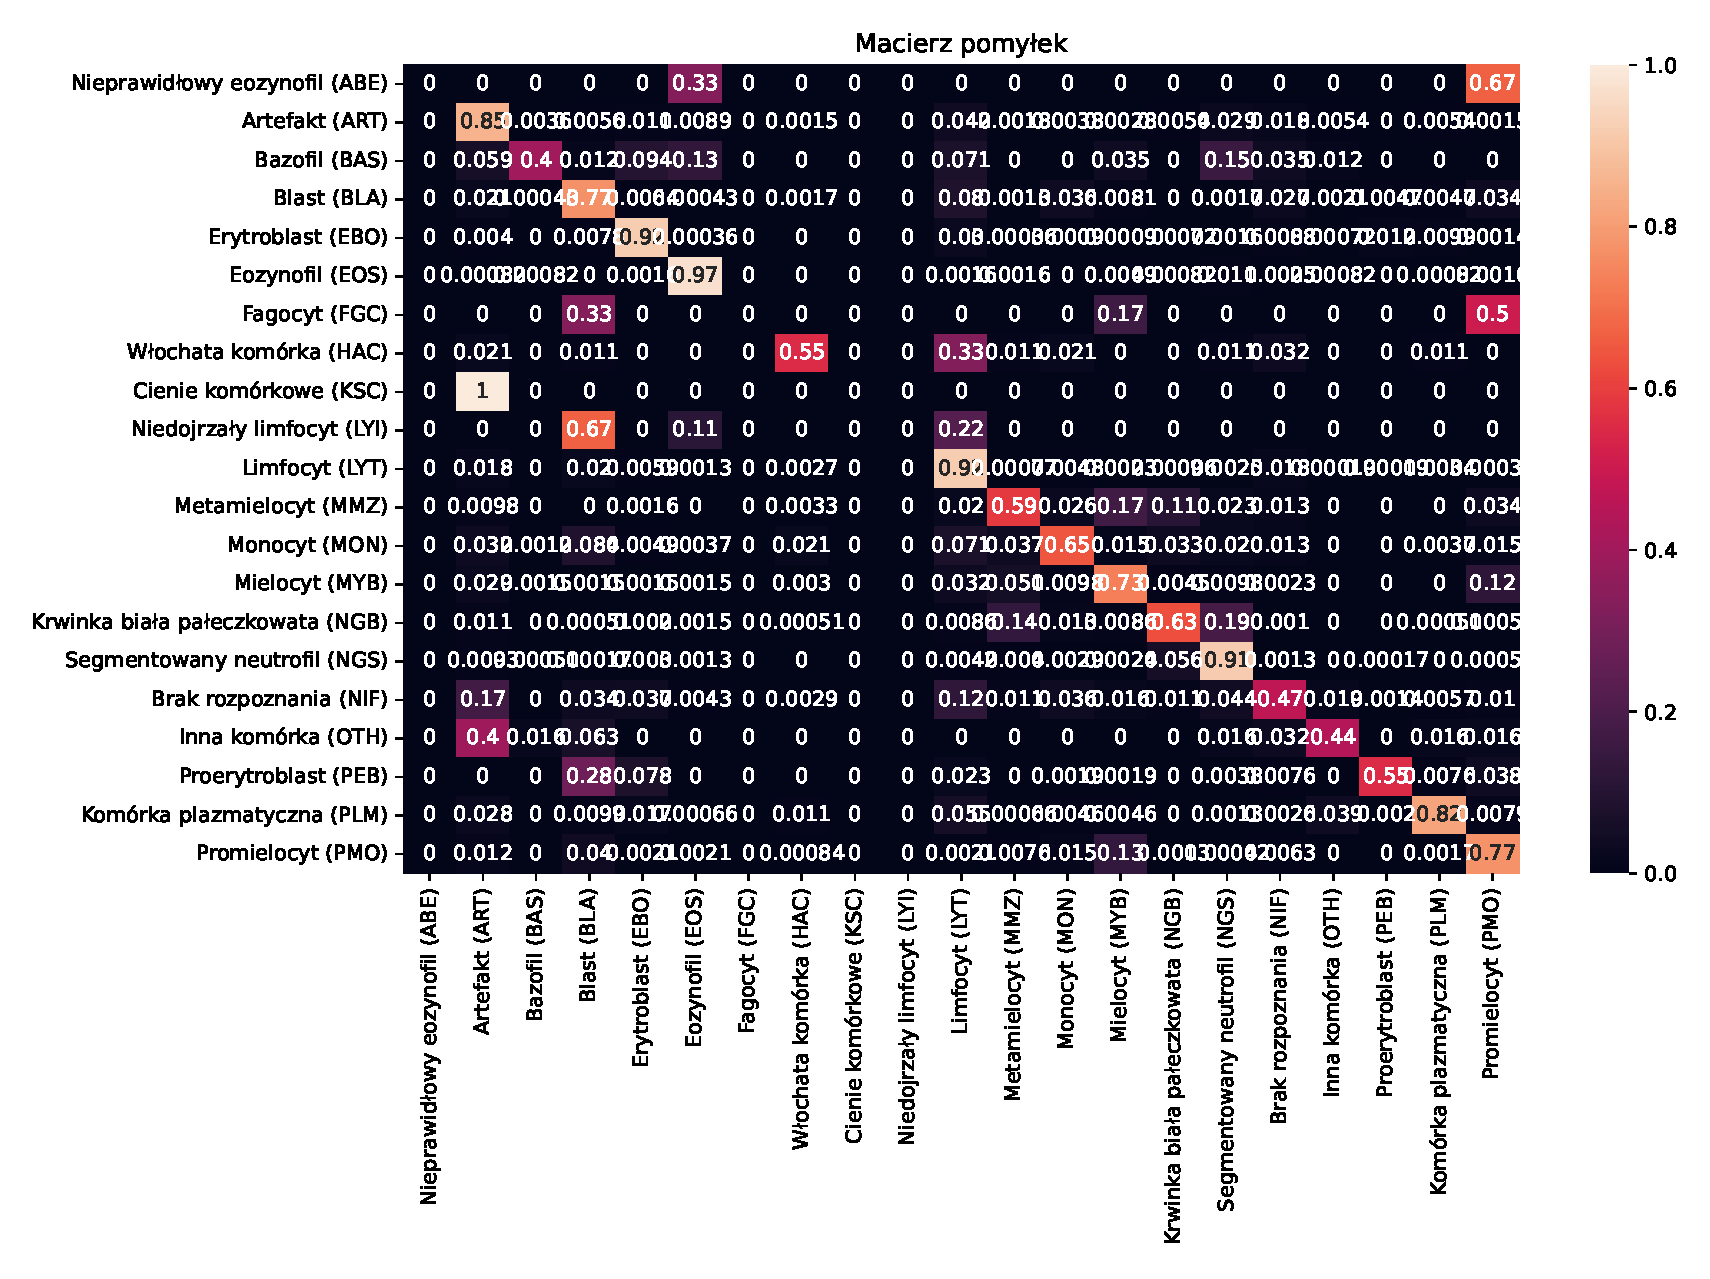
\includegraphics[width=\textwidth]{experiments/efficientnet_b0/confusion_matrix}
    \caption{Macierz pomyłek dla najlepszego modelu}
\end{figure}

\begin{figure}
    \centering
    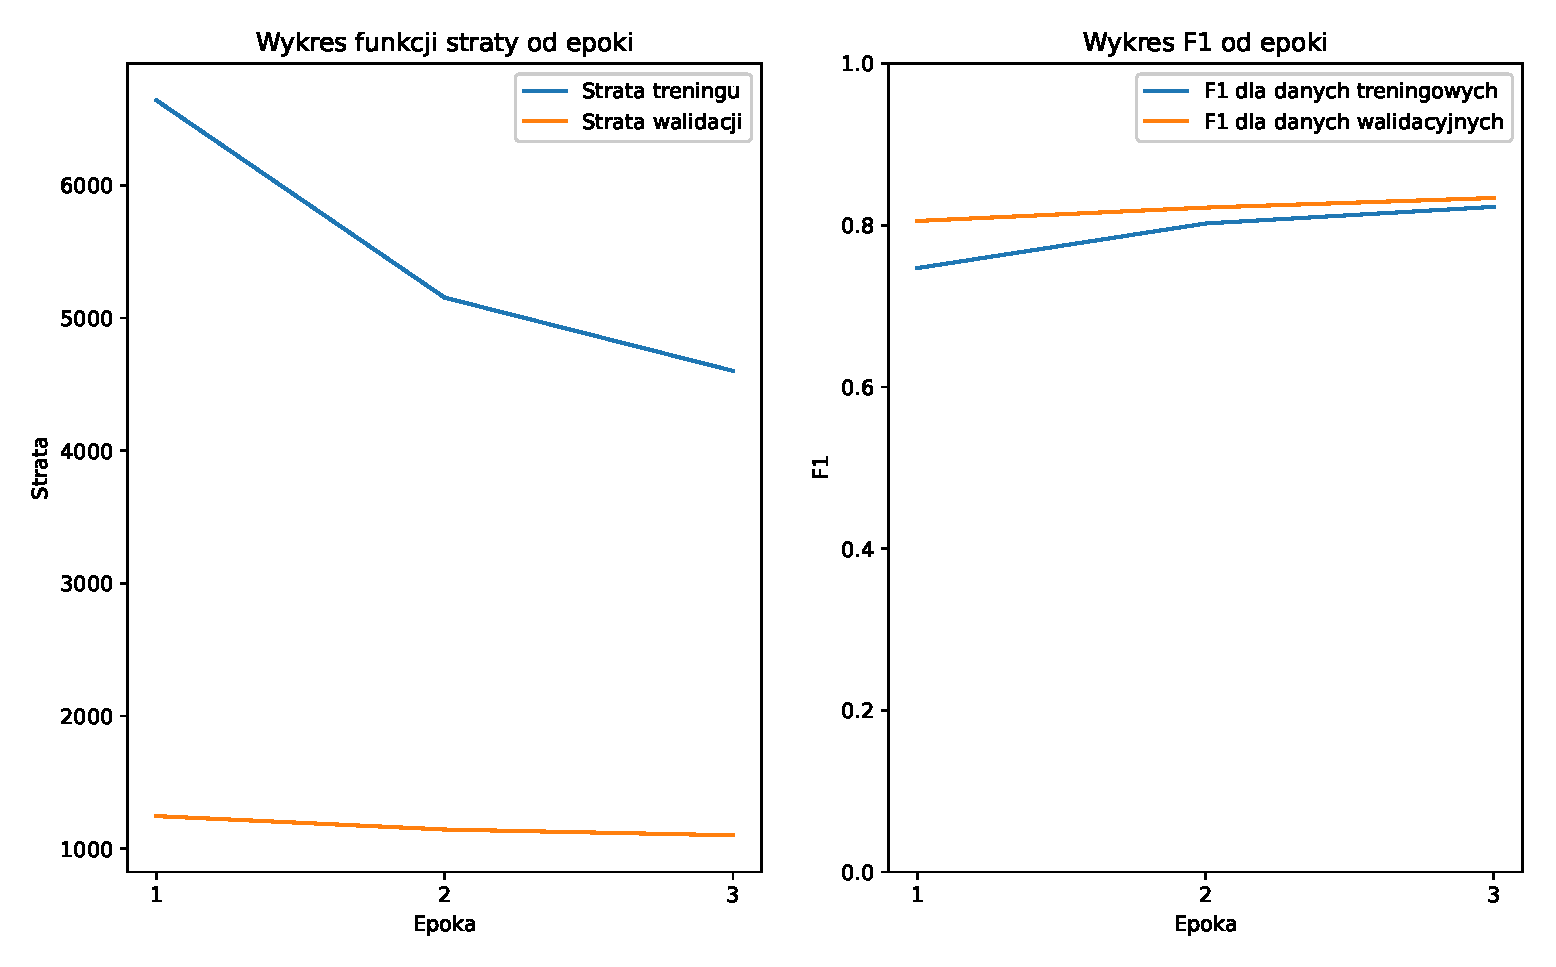
\includegraphics[width=\textwidth]{experiments/efficientnet_b0/combined}
    \caption{Wykres zależności funkcji straty i F1 od epoki trenowania}
\end{figure}

\begin{figure}
    \centering
    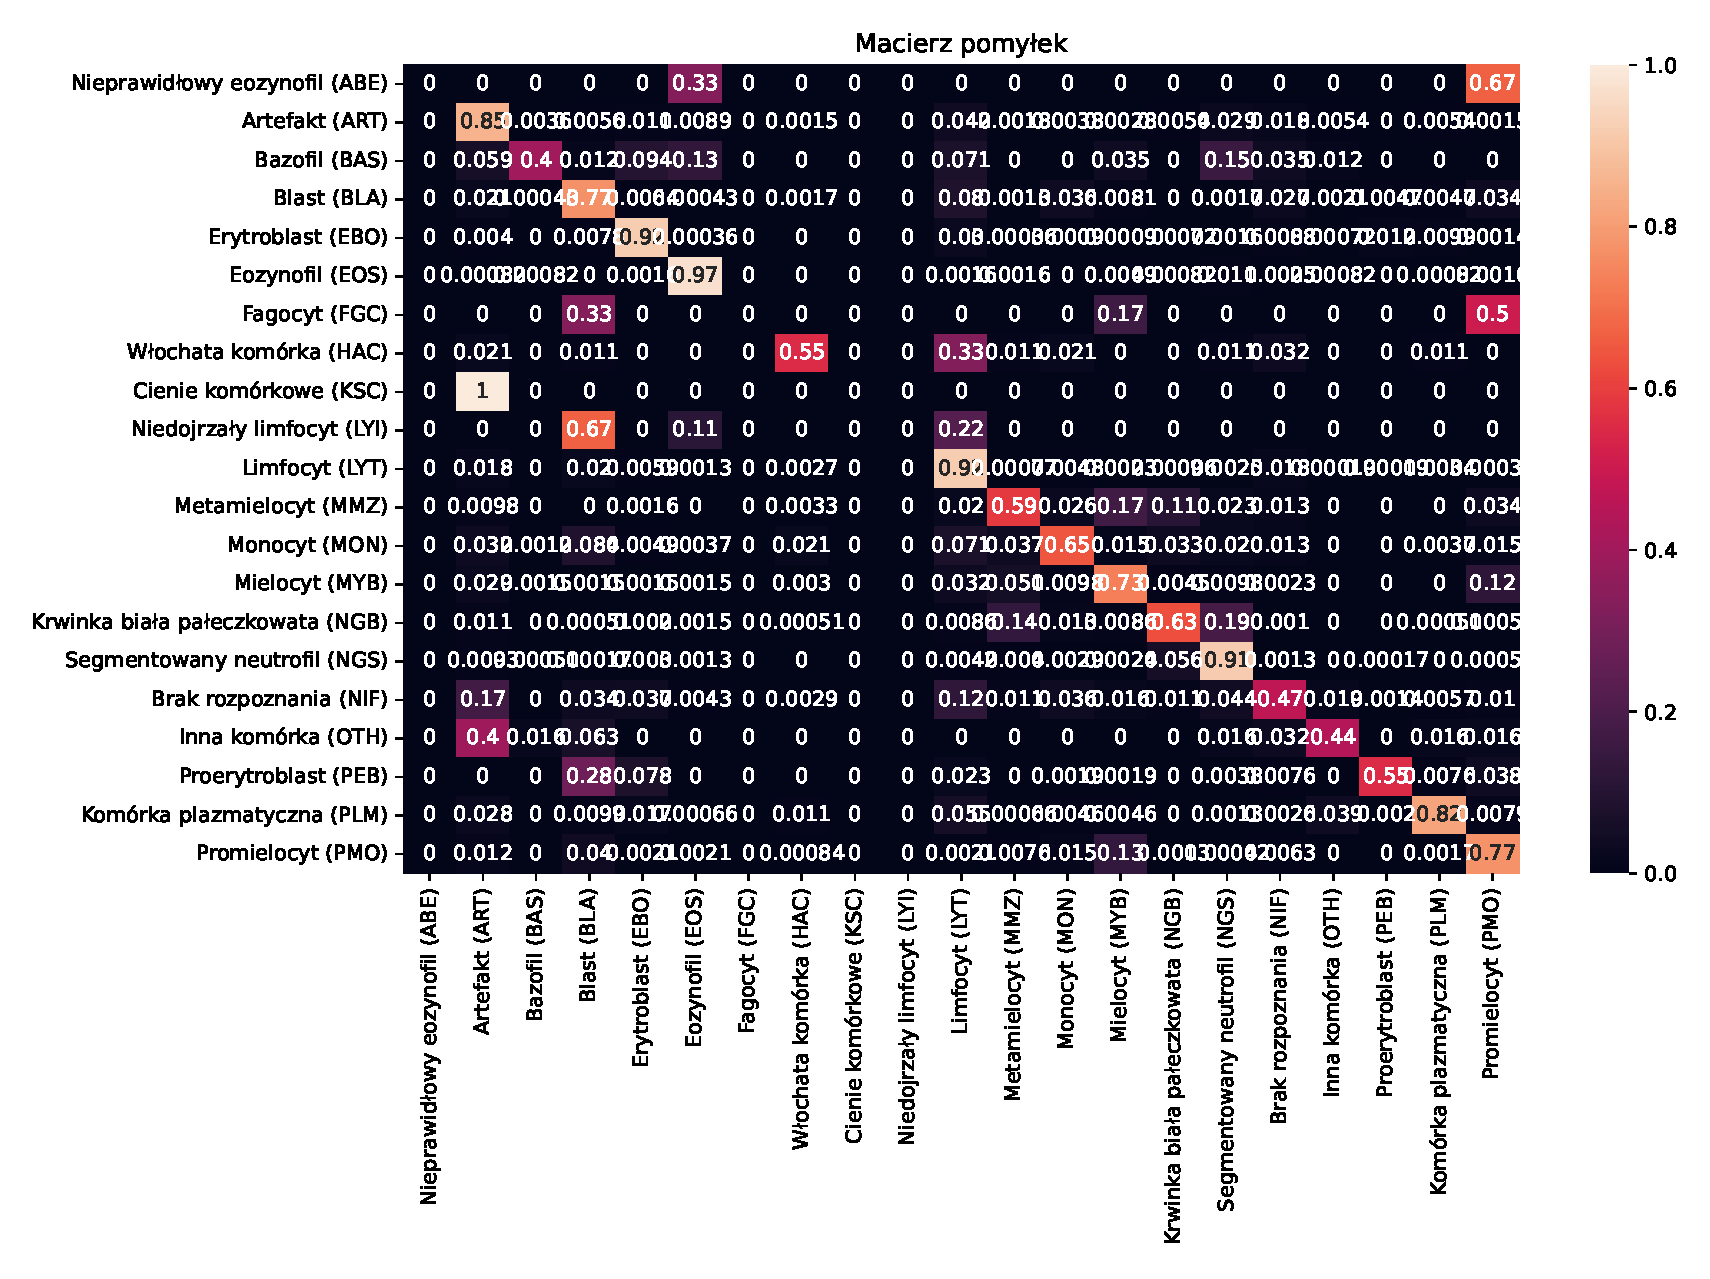
\includegraphics[width=\textwidth]{experiments/efficientnet_b0/confusion_matrix}
    \caption{Macierz pomyłek dla najlepszego modelu}
\end{figure}

%TODO end 9 listings


%TODO choose best architecture
Najlepsze wyniki uzyskuje model używający architektury \textit{EfficientNet B0}. Ważony wynik F1 w jej przypadku wynosi \textit{0.86}.
Tabela \ref{tab:f1_summary} przedstawia zestawienie precyzji, czułości i F1 dla poszczególnych klas.
Z kolei wykresy na rys. \ref{fig:plot} przedstawiają zależności funkcji straty i F1 od epoki trenowania.
Można stwierdzić, że jakość modelu nie poprawia się zbyt znacząco wraz z kolejnymi iteracjami.
Macierz pomyłek jest widoczna natomiast na rys. \ref{fig:confusion_matrix}.
Informuje ona, które klasy są najczęściej mylone z którymi.

\section{Porównanie z innymi algorytmami}

\begin{figure}
    \centering
    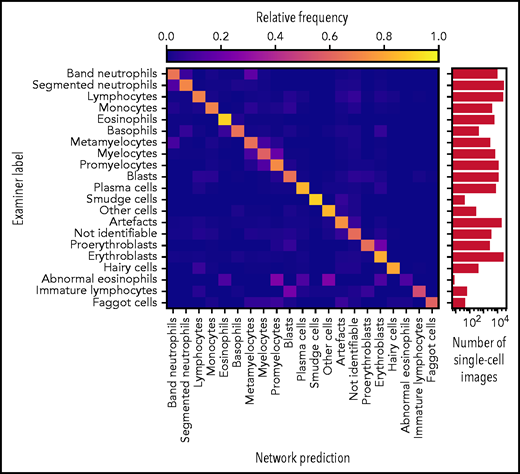
\includegraphics[width=\textwidth]{resnext_confusion_matrix}
    \caption{Macierz pomyłek dla modelu ResNeXt}
    \label{fig:resnext_confusion_matrix}
\end{figure}

Dostawca zbioru danych, w artykule \textit{Highly accurate differentiation of bone marrow cell morphologies using deep neural networks on a large image dataset} \cite{resnext} wykorzystuje architekturę \textit{ResNetXt-50}.
Model zawierający ponad 23 miliony parametrów był trenowany na \textit{NVIDIA TESLA V100} przez ok. 48 godzin.
Podobnie jak w niniejszej pracy, autorzy artykułu wykonali normalizację intensywności kolorów przed trenowaniem sieci neuronowej (z powodu różnic w barwieniu Maya-Grünwalda-Giemsa).
Uzyskany ważony wynik F1 dla architektury \textit{ResNeXt-50} wyniósł \textit{0.822}. Macierz pomyłek dostarczona przed autorów pracy jest widoczna na rys. \ref{fig:resnext_confusion_matrix}.

\section{Wyzwania}

Głównym wyzwaniem napotkanym w projekcie było wytrenowanie dużych sieci neuronowych. Niestety, ich trening na lokalnym sprzęcie takim jak komputer osobisty jest bardzo czasochłonne.
W związku z tym konieczne było uruchamianie ich na platformie \textit{kaggle.com}, która oferuje 30 godzin czasu procesora graficznego miesięcznie.
Ten górny limit wymuszał przemyślane zarządzanie tym, która sieć neuronowa powinna być wytrenowana priorytetowo.

\section{Wnioski}

%TODO net
Zaprezentowane porównanie różnych splotowych sieci neuronowych informuje, że najlepszym modelem do zadania klasyfikacji rodzajów komórek w szpiku kostnym jest \textit{EfficientNet B0}.
Ta sieć neuronowa uzyskuje najlepszy ważony wynik F1 równy \textit{0.866}.
Warto też zwrócić uwagę na to, że sieci neuronowe znacznie większe od \textit{EfficientNet B0} nie dawały dużo lepszych rezultatów.

\section{Perspektywy rozwoju projektu}

Jedną z możliwości poprawienia jakości modelu jest zrównoważenie zbioru danych, by każda z klas zawierała podobną, dużą ilość próbek.

